%%%%%%%%%%%%%%%%%%%%%%%%%%%%%%%%%%%%%%%%%%%%%%%%%%%%%%%%
%%        OPUS Document Ganerator
%%        Project report: myprop
%%
%%        Computer Engineering Project
%%        Department of Computer Engineering
%%        Faculty of Engineering at Sri Racha
%%        Kasetsart University, Sri Racha Campus
%%%%%%%%%%%%%%%%%%%%%%%%%%%%%%%%%%%%%%%%%%%%%%%%%%%%%%%%
\documentclass[12pt,a4paper,oneside]{book}
\usepackage{fontspec}
\usepackage{xunicode}
\usepackage{xltxtra}
\usepackage{graphicx}
\usepackage{tabularx}
\usepackage{lastpage}
\usepackage{titlesec}
\usepackage{fancyvrb}
\usepackage{amsmath}
\usepackage{url}
\usepackage{float}
\usepackage{indentfirst}
\usepackage{listings}
\usepackage[font=large, labelfont=bf]{caption}
\setmainfont[Scale=1.23,Path=fonts/,UprightFont=*-Regular,BoldFont=*-Bold,ItalicFont=*-Italic,BoldItalicFont=*-BoldItalic]{THSarabunNew}
\titleformat{\chapter}[display]{\Huge\bfseries\centering}{\chaptertitlename\ \thechapter}{20pt}{}
\defaultfontfeatures{Scale=1.23}
\XeTeXlinebreaklocale{th_TH}
\newcommand{\thi}{\fontspec[Scale=1.23,Path=fonts/,UprightFont=*-Regular,BoldFont=*-Bold,ItalicFont=*-Italic,BoldItalicFont=*-BoldItalic]{THSarabunNew}}
\newcommand\thisYear{\advance\year by 543 \the\year\advance\year by -543}
\renewcommand{\contentsname}{{\thi สารบัญ}}
\renewcommand{\listtablename}{{\thi สารบัญตาราง}}
\renewcommand{\listfigurename}{{\thi สารบัญภาพ}}
\renewcommand{\chaptername}{{\thi บทที่}}
\renewcommand{\figurename}{{\thi ภาพที่}}
\renewcommand{\tablename}{{\thi ตารางที่}}
\renewcommand{\appendixname}{{\thi ภาคผนวก}}
\renewcommand{\bibname}{{\thi เอกสารและสิ่งอ้างอิง}}

\linespread{1.2}
\setlength{\textwidth}{5.8in}
\setlength{\topmargin}{-0.5in}
\setlength{\oddsidemargin}{0.5in}
\setlength{\parskip}{0.2in}
\setlength{\parindent}{0.5in}
\setlength{\textheight}{9.0in}
\setlength{\footskip}{0.5in}
\graphicspath{{./images/}}

%%%%%%%%%%%%%%%%%%% Document Start %%%%%%%%%%%%%%%%%%%%%
\begin{document}
%Set the same font for Thai and English.
%\fontspec[Scale=1.23,Path=fonts/,UprightFont=*-Regular,BoldFont=*-Bold,ItalicFont=*-Italic,BoldItalicFont=*-BoldItalic]{THSarabunNew}

\pagestyle{myheadings}
\pagenumbering{gobble}
{
\fontsize{14pt}{16pt}\selectfont
%%%%%%%%%%%%%%%%%%%%% Main Cover %%%%%%%%%%%%%%%%%%%%%%%
\begin{center}

\includegraphics[scale=0.25]{ku_black.jpg}

{\fontsize{35pt}{37pt}\selectfont\bfseries {\thi โครงงานวิศวกรรมคอมพิวเตอร์}}

\vspace{0.3in}
{\fontsize{20pt}{22pt}\selectfont\bfseries {\thi ระบบควบคุมเครื่องใช้ไฟฟ้าในบ้านผ่านแอปพลิเคชั่น}

Electronics Control System by Application}
\vfill
{\fontsize{20pt}{22pt}\selectfont\bfseries
{\thi นายตรีธนพงศ์} {\thi เอี่ยมรอด}\\
{\thi นายธนวัฒน์} {\thi พลชัย}
}
\vfill
{\fontsize{20pt}{22pt}\selectfont\bfseries {\thi ภาควิชาวิศวกรรมคอมพิวเตอร์} {\thi คณะวิศวกรรมศาสตร์ศรีราชา}\\
{\thi มหาวิทยาลัยเกษตรศาสตร์} {\thi วิทยาเขตศรีราชา}\\
{\thi พ}.{\thi ศ}. \thisYear}\\
\end{center}

%%%%%%%%%%%%%%%%%%%% Inside Cover %%%%%%%%%%%%%%%%%%%%%%
\newpage
\begin{center}
{\thi โครงงานวิศวกรรมคอมพิวเตอร์}

{\thi เรื่อง}

{\thi ระบบควบคุมเครื่องใช้ไฟฟ้าในบ้านผ่านแอปพลิเคชั่น}

Electronics Control System by Application
\vfill
{\thi โดย}

{\thi นายตรีธนพงศ์} {\thi เอี่ยมรอด}\\
{\thi นายธนวัฒน์} {\thi พลชัย}

\vfill
{\thi เสนอ}

{\thi ภาควิชาวิศวกรรมคอมพิวเตอร์} {\thi คณะวิศวกรรมศาสตร์ศรีราชา}\\
{\thi มหาวิทยาลัยเกษตรศาสตร์} {\thi วิทยาเขตศรีราชา}\\
{\thi เพื่อความสมบูรณ์แห่งปริญญาวิศวกรรมศาสตรบัณฑิต} ({\thi วิศวกรรมคอมพิวเตอร์})\\
{\thi พ}.{\thi ศ}. \thisYear
\end{center}

%%%%%%%%%%%%%%%%%%%% Approval Form %%%%%%%%%%%%%%%%%%%%%
\newpage
\begin{center}
\textbf{
{\thi ปริญญาวิศวกรรมศาสตรบัณฑิต} ({\thi วิศวกรรมคอมพิวเตอร์})
}

\textbf{{\thi ภาควิชาวิศวกรรมคอมพิวเตอร์} \hfill {\thi คณะวิศวกรรมศาสตร์ศรีราชา}}
\end{center}
\vfill
\begin{tabular}{ll}
\textbf {\thi เรื่อง} & {\thi ระบบควบคุมเครื่องใช้ไฟฟ้าในบ้านผ่านแอปพลิเคชั่น} \\
& Electronics Control System by Application \\
\\
\textbf {\thi นามผู้จัดทำ} &
{\thi นายตรีธนพงศ์} {\thi เอี่ยมรอด}\\
&{\thi นายธนวัฒน์} {\thi พลชัย}
\end{tabular}
\vfill
\begin{center}
\begin{tabularx}{\textwidth}{lX}
\textbf {\thi ได้รับพิจารณาเห็นชอบโดย} & \\
\\
{\thi อาจารย์ที่ปรึกษาโครงงานหลัก} & \dotfill\ \\
& \centerline{({\thi อาจารย์วัชรพัฐ} {\thi เมตตานันท})} \\
{\thi กรรมการโครงงาน} & \dotfill\ \\
& \centerline{({\thi อาจารย์ปุณณะ} {\thi ยศปัญญา})} \\
{\thi กรรมการโครงงาน} & \dotfill\ \\
& \centerline{({\thi อาจารย์วัลลภ} {\thi อินทร์ฉ่ำ})} \\
\end{tabularx}
\begin{tabularx}{\textwidth}{Xc}
& \textbf{{\thi ภาควิชาวิศวกรรมคอมพิวเตอร์} {\thi คณะวิศวกรรมศาสตร์ศรีราชา}}\\
& \textbf{{\thi มหาวิทยาลัยเกษตรศาสตร์} {\thi วิทยาเขตศรีราชา} {\thi รับรองแล้ว}}\\
& \\
& \dotfill\ \\
& ({\thi อาจารย์วัชรพัฐ} {\thi เมตตานันท}) \\
& {\thi หัวหน้าภาควิชาวิศวกรรมคอมพิวเตอร์} \\
& \\
& {\thi วันที่} \dotfill\ \\
\end{tabularx}

\end{center}

%%%%%%%%%%%%%%%%%%%%% Abstract TH %%%%%%%%%%%%%%%%%%%%%%
\newpage
\begin{quote}
{\thi นายตรีธนพงศ์} {\thi เอี่ยมรอด}, {\thi นายธนวัฒน์} {\thi พลชัย}, \thisYear: {\thi ระบบควบคุมเครื่องใช้ไฟฟ้าในบ้านผ่านแอปพลิเคชั่น}, {\thi ปริญญาวิศวกรรมศาสตรบัณฑิต} ({\thi วิศวกรรมคอมพิวเตอร์}) {\thi ภาควิชาวิศวกรรมคอมพิวเตอร์} {\thi คณะวิศวกรรมศาสตร์ศรีราชา}, {\thi อาจารย์ที่ปรึกษาโครงงานหลัก}: {\thi อาจารย์วัชรพัฐ} {\thi เมตตานันท}, {\thi วศ}.{\thi ม}. \pageref{LastPage} {\thi หน้า}
\end{quote}
\vspace{0.2in}
\begin{center}
\textbf{\Huge {\thi บทคัดย่อ}}
\end{center}
\vspace{0.3in}
\hspace{-0.5in}

{\thi โครงงานนี้นำเสนอระบบควบคุมเครื่องใช้ไฟฟ้าภายในบ้าน} {\thi ผ่านแอปพลิเคชัน} {\thi โดยพัฒนาในแบบโมบายแอปพลิเคชันและชุดวงจรควบคุมระบบ} {\thi ระบบงานนี้ใช้โปรแกรม} Android Studio {\thi ในการออกแบบแอปพลิเคชั่นในระบบปฏิบัติการแอนดรอยด์} {\thi ภาษาไพทอน}, {\thi จาวา} {\thi จาวาสคริปต์และภาษาซีในการพัฒนาระบบ} {\thi และมี} Raspberry PI {\thi เพื่อควบคุมอุปกรณ์ไฟฟ้า} 3 {\thi รูปแบบ} {\thi ได้แก่} {\thi อุปกรณ์ที่สั่งด้วยสัญญาณอินฟาเรด}, {\thi อุปกรณ์ที่ต่อกับสวิตซ์ไฟ} {\thi และผ้าม่าน} {\thi โดยมุ่งหวังว่า} {\thi จะเป็นการเพิ่มช่องทางในการควบคุมระบบเครื่องใช้ไฟฟ้าภายในบ้าน}  

{\thi ผลการดำเนินโครงการพบว่าระบบที่พัฒนาขึ้น} {\thi สามารถทำงานได้ตรงตามขอบเขตที่ได้กำหนดไว้} {\thi และได้ทำการทดสอบความพึงพอใจกับกลุ่มตัวอย่างผู้ใช้งานจำนวน} 30 {\thi คน} {\thi โดยใช้แบบสอบถาม} {\thi ผล} {\thi การวัดความพึงพอใจพบว่า} {\thi ผู้ใช้งานมีความพึงพอใจค่อนข้างดี}


%%%%%%%%%%%%%%%%%%%%% Abstract EN %%%%%%%%%%%%%%%%%%%%%%
\newpage
\begin{quote}
Threetanaphong Iamrod, Tanawat Ponchai, \the\year: Electronics Control System by Application, Bachelor of Engineering (Computer Engineering), Department of Computer Engineering, Faculty of Engineering at Siracha, Project Advisor: Vacharapat Mettanant, M.Eng. \pageref{LastPage} pages
\end{quote}
\vspace{0.2in}
\begin{center}
\textbf{\Huge Abstract}
\end{center}
\vspace{0.3in}
\hspace{-0.5in}

This research project is presentations. An electric appliance control system via application. The development of the mobile applications. This system uses the Android Studio, Python, Java JavaScript and C for design application interface and uses the Raspberry pi for control three type of electronics such as control with infrared signal, electronics connect to switch and curtain. With the aim is to increase the way to control the electric appliance in home.

The results showed that the developed system can be used to meet the specified limits and satisfaction were tested with a sample of 30 users, using a questionnaire. The results showed that satisfaction. User satisfaction is quite good.


%%%%%%%%%%%%%%%%%%%%% Acknowledgement %%%%%%%%%%%%%%%%%%%%%%
\chapter*{{\thi กิตติกรรมประกาศ}}

{\thi การดำเนินโครงงาน} {\thi ระบบควบคุมเครื่องใช้ไฟฟ้าในบ้านผ่านแอปพลิเคชั่น} {\thi จะไม่สามารถสำเร็จลุล่วงได้ด้วยดี} {\thi หากขาดการสนับสนุนและกำลังจากหลายๆ} {\thi ฝ่าย} {\thi อาทิ}

{\thi อาจารย์อาจารย์วัชรพัฐ} {\thi เมตตานันท} {\thi อาจารย์ที่ปรึกษาโครงงาน} {\thi สำหรับคำปรึกษา} {\thi คำแนะนำ} {\thi และแนวทางการแก้ไขเมื่อเกิดปัญหาในการพัฒนาโครงงาน}

{\thi คุณพ่อ} {\thi คุณแม่} {\thi และครอบครัว} {\thi ที่คอยไต่ถาม} {\thi เฝ้าติดตามการพัฒนาโครงงานด้วยความห่วงใย} {\thi และมอบกำลังใจในยามที่เกิดปัญหา}

{\thi นิสิตภาควิชาวิศวกรรมคอมพิวเตอร์} {\thi คณะวิศวกรรมศาสตร์​ศรีราชา} {\thi มหาวิทยาลัยเกษตรศาสตร์} {\thi วิทยาเขตศรีราชา} {\thi ปีการศึกษา} 2559
{\thi ที่ช่วยทดสอบและแจ้งปัญหาจากการใช้งาน} {\thi รวมทั้งคำแนะนำเพิ่มเติมที่มีประโยชน์ต่อการพัฒนาโครงงาน}

{\thi ผู้จัดทำใคร่ขอขอบพระคุณทุกท่านเป็นอย่างสูง} {\thi ณ} {\thi ที่นี้ที่ได้ช่วยให้การดำเนินโครงงานในครั้งนี้สำเร็จลุล่วงไปได้ด้วยดี}

\begin{flushright}
{\thi นายตรีธนพงศ์} {\thi เอี่ยมรอด}\\
{\thi นายธนวัฒน์} {\thi พลชัย}\\
{\thi พฤษภาคม} \thisYear
\end{flushright}

%%%%%%%%%%%%%%%%%% Table of Contents %%%%%%%%%%%%%%%%%%%
\newpage
\pagenumbering{roman}
\tableofcontents
\listoftables
\listoffigures

%%%%%%%%%%%%%%%%%%%%%% Contents %%%%%%%%%%%%%%%%%%%%%%%%
\newpage
\pagenumbering{arabic}
%%%%%%%%%%%%%%%%% {\thi บทนำ} %%%%%%%%%%%%%%%%%%%
\chapter{{\thi บทนำ}}


\section{{\thi ความเป็นมา}}


{\thi วิถีชีวิตประจำวันของมนุษย์ในปัจจุบันมีการใช้ชีวิตประจำวันที่เร่งรีบและมีการแข่งขันสูงอาจทำให้เกิดการผิดพลาดในการตรวจสอบการปิดเครื่องใช้ไฟฟ้าต่าง} {\thi ๆ} {\thi ก่อนที่จะออก}
{\thi เดินทาง} {\thi ก่อให้เกิดปัญหาการสิ้นเปลืองไฟฟ้าและอาจก่อให้เกิดอัคคีภัยจากเครื่องใช้ไฟฟ้าได้} {\thi เทคโนโลยีต่าง} {\thi ๆ} {\thi ในปัจจุบันได้เข้ามามีบทบาทในการใช้ชีวิตประจำวันอย่างมากมาย}  {\thi จึงต้องหาเครื่องมือหรือเครื่องใช้ที่ทำให้เกิดความสะดวกสบายในการดำรงชีวิตมีความปลอดภัยและสามารถช่วยลดค่าใช้จ่ายต่าง} {\thi ๆ} {\thi ได้} {\thi ซึ่งทำให้มนุษย์มีคุณภาพชีวิตที่ดีขึ้นเพื่อให้ทันต่อการใช้ชีวิตและยังใช้เทคโนโลยีให้เกิดประโยชน์อีกด้วย} {\thi เราจึงจัดทำระบบควบคุมเครื่องใช้ไฟฟ้าในบ้านผ่านแอปพลิเคชั่น}(Application)


\section{{\thi วัตถุประสงค์}}


{\thi เพื่อพัฒนาระบบควบคุมเครื่องใช้ไฟฟ้าและพัฒนาแอปพลิเคชันสำหรับระบบปฎิบัติแอนดรอยด์}(Android){\thi โดยสั่งผ่านโมบายแอปพลิเคชันได้}  3 {\thi รูปแบบ}
\begin{enumerate}
\item{{\thi อุปกรณ์ที่สั่งด้วยสัญญาณอินฟาเรด}}
\item{{\thi อุปกรณ์ที่ต่อกับสวิตซ์ไฟ}}
\item{{\thi ผ้าม่าน}}
\end{enumerate}


\section{{\thi ขอบเขตของโครงงาน}}

\begin{enumerate}
\item{{\thi แอปพลิเคชันสามารถควบคุมอุปกรณ์ไฟฟ้า} {\thi แอร์} {\thi ทีวี} {\thi ผ้าม่านกันแสง} {\thi เครื่องใช้ไฟฟ้าที่ต่อกับสวิตซ์ปิดเปิดไฟและสามารถเช็คอุณหภูมิได้}}
\item{{\thi ระบบปฏิบัติการแอนดรอยด์สามารถควบคุมอุปกรณ์ไฟฟ้าได้ผ่านเสียง}}
\item{{\thi ระบบปฏิบัติการไอโอเอส}(iOS){\thi สามารถควบคุมอุปกรณ์ไฟฟ้าผ่านเสียงได้โดยใช้} Siri}
\item{{\thi แอปพลิเคชันสามารถสั่งปิดอุปกรณ์ไฟฟ้าอัตโนมัติในกรณีไม่มีคนอยู่เป็น} schedule}
\item{{\thi แอปพลิเคชันสามารถสร้างฉาก}(Scene){\thi ที่รวมคำสั่งควบคุมอุปกรณ์หลายคำสั่งไว้ด้วยกันได้}}
\item{{\thi แอปพลิเคชันสามารถตั้งเงื่อนไขในการสั่งการอัตโนมัติได้สำหรับแอนดรอยด์}}

\end{enumerate}

\section{{\thi ประโยชน์ที่ได้รับ}}

\begin{enumerate}
\item{{\thi เพื่ออำนวยความสะดวกในการใช้เครื่องใช้ไฟฟ้า}}
\item{{\thi เพื่อลดปัญหาการลืมปิดอุปกรณ์ไฟฟ้า}}
\item{{\thi เพื่อประหยัดค่าใช้จ่าย}}
\item{{\thi เพื่อเพิ่มความปลอดภัยให้มากขึ้น}}
\item{{\thi เพื่อลดเวลาในการใช้งาน}}
\end{enumerate}

\section{{\thi กลุ่มผู้ใช้งาน}}
{\thi ผู้ที่อาศัยอยู่ในคอนโดมิเนียมหรือบ้านขนาดเล็ก}

\section{{\thi แผนการดำเนินงาน}}

\begin{enumerate}
\item{{\thi ศึกษาระบบงานและเทคโนโลยีที่ใช้ในการพัฒนา}}
\item{{\thi การนำเสนอโครงงาน}}
\item{{\thi การวิเคราะห์ระบบงาน}}
\item{{\thi วางแผนออกแบบระบบงาน}}
\item{{\thi พัฒนาโปรแกรมที่ได้ออกแบบ}}
\item{{\thi ทดสอบระบบการทำงาน}}
\item{{\thi ปรับปรุงและแก้ไขข้อผิดพลาดของระบบ}}
\item{{\thi สรุปและจัดทำเอกสารประกอบโครงงาน}}
\end{enumerate}

%%%%%%%%%%%%%%%%% {\thi ความรู้พื้นฐานและงานที่เกี่ยวข้อง} %%%%%%%%%%%%%%%%%%%
\chapter{{\thi ความรู้พื้นฐานและงานที่เกี่ยวข้อง}}



{\thi ในการดำเนินการจัดทำโครงการ} {\thi เรื่อง} {\thi ระบบควบคุมเครื่องใช้ไฟฟ้าภายในบ้านผ่านแอปพลิเคชัน} {\thi ผู้จัดทำได้ทำศึกษาหลักการทฤษฏี} {\thi และเทคโนโลยีต่าง} {\thi ๆ} {\thi ที่เกี่ยวข้องกับ}
{\thi ความสามารนำมาประยุกต์ใช้ในการพัฒนาระบบ} {\thi ซึ่งประกอบไปด้วยหัวข้อต่าง} {\thi ๆ} {\thi ดังนี้}

\section{Python Language}
	{\thi ภาษาไพธอน}(Python){\thi เป็นภาษาโปรแกรมคอมพิวเตอร์ระดับสูงที่มีโครงสร้างของภาษาที่ไม่ซับซ้อนทำให้ง่ายต่อการเรียนรู้} {\thi และสามารถทำงานร่วมกับภาษาโปรแกรมอื่น} {\thi ๆ} {\thi ได้หลายภาษา} {\thi และยังเป็นภาษาสคริปต์} (Scripting Language){\thi ทำให้ใช้เวลาในการเขียนและคอมไพล์ไม่มาก} {\thi นอกจากนี้ยังมีเฟรมเวิร์ค}(Framework){\thi ที่สามารถใช้สร้างเว็บเซอร์วิส}(Web Service){\thi ได้คือ} Flask Framework
	\subsection{Flask Framework}
	Flask {\thi เป็นเฟรมเวิร์คหนึ่งของภาษาไพธอน} {\thi ที่ช่วยให้เราสามารถเขียน} python web application {\thi ได้} {\thi ซึ่งจุดเด่นของ} Flask {\thi คือความเรียบง่ายและความยืดหยุ่น} {\thi และเหมาะสำหรับแอพพลิ}-{\thi เคชั่นที่ทำงานหน้าเดียว} {\thi โดยจะมีตัวอย่างดังนี้} 
	
	\newpage

	\lstset{basicstyle=\footnotesize\ttfamily,breaklines=true}\begin{lstlisting}[frame=single]
from flask import Flask
app = Flask(__name__)

@app.route("/on_air/")
def on_air():
   rtn =subprocess.call(["irsend", "SENDONCE", "REMOTEAIR", "AIRON"])

if __name__ == "__main__":
    app.run(host='0.0.0.0')

\end{lstlisting}

{\thi จากตัวอย่างด้านบน} {\thi เมื่อรันแล้วจะได้เว็บเซอร์วิสที่สามรถเรียกใช้ผ่าน} URL {\thi เช่นต้องการเรียกใช้งานฟังก์ชัน}(Function) on\_air {\thi ก็สามารถเรียก} http://<ip address>:5000/on\_air {\thi และหากต้องการเพิ่มการเรียกใช้งานเพิ่มเติม} {\thi ก็สารามารถเพิ่ม} @app.route("/path{\thi ที่ต้องการ}") {\thi ได้เลย} 

\section{Android}
	{\thi แอนดรอยด์เป็นระบบปฏิบัติการบนอุปกรณ์พกพาซึ่งเป็นแบบโอเพนซอร์ซ}(Open Source) {\thi โดยสามารถนำไปพัฒนาเพิ่มเติมเสริมแต่งได้} {\thi โดยสามารถสร้างแอปพลิเคชันจากภาษาโปรแกรมจาวา}(Java) {\thi และภาษาโปรแกรมเอกซ์เอ็มแอล}(XML)
	 \subsection{Java Language}
	{\thi ภาษาจาวาเป็นภาษาสำหรับเขียนโปรแกรมที่สนับสนุนการเขียนโปรแกรมเชิงวัตถุ} (OOP:Object-Oriented Programming) {\thi โดยโปรแกรมที่เขียนขึ้นถูกสร้างภายในคลาส}(Class) {\thi และแต่ละคลาสคือที่เก็บเมทอด}(Method) {\thi โดยสามารถใช้เขียนในส่วนของการทำงานในแอปพลิเคชันได้} {\thi ซึ่งใช้} Android Studio {\thi ในการพัฒนา}

	\subsection{XML Language}
	{\thi ภาษาเอกซ์เอ็มแอล}(Extensible Markup Language) {\thi ใช้กำหนดภาพแบบของคำสั่งภาษาแบบ} Meta Data {\thi ซึ่งมีโครงสร้างที่ประกอบด้วยแท็กเปิด} {\thi และแท็กปิด} {\thi เช่นเดียวกับภาษา} HTML {\thi แต่ภาษา} XML {\thi คุณสามารถสร้างแท็กรวมทั้งกำหนดโครงสร้างของข้อมูลได้เอง} {\thi ซึ่งสามารถนำไปใช้ในการสร้าง} layout {\thi ของแอนดรอยด์แอปพลิเคชันได้}

\subsection{ListView}
	ListView {\thi เป็น} {\thi ไลบรารี่}(Library) {\thi ที่ช่วยจัดการในการแสดงข้อมูลที่เป็นลิสต์}(List) {\thi ให้แสดงเป็นแถว}(Row) {\thi ซึ่งแต่ละแถวจะมี} layout {\thi ตามที่ออกแบบไว้} {\thi โดยมีตัวอย่างดังนี้}

{\thi โค้ดตัวอย่างของการจองพื้นนี้ให้} listview {\thi ในไฟล์} .xml
\lstset{basicstyle=\footnotesize\ttfamily,breaklines=true}\begin{lstlisting}[frame=single]
<ListView
            android:id="@+id/listView"
            android:layout_width = "500dp"
            android:layout_height ="500dp">
</ListView>
\end{lstlisting}

{\thi โค้ดตัวอย่างของการจัดการการแสดงผลใน} listview
\lstset{basicstyle=\footnotesize\ttfamily,breaklines=true}\begin{lstlisting}[frame=single]
public class listAdapter extends BaseAdapter {
    @Override
    public int getCount() {
        return 0;
    }

    @Override
    public Object getItem(int position) {
        return null;
    }

    @Override
    public long getItemId(int position) {
        return 0;
    }

    @Override
    public View getView(int position, View convertView, ViewGroup parent) {
        return null;
    }
}
\end{lstlisting}
 
\newpage
{\thi โค้ดตัวอย่างของการเรียกใช้} listview {\thi มาทำงานในภาษาจาวาและแสดงผล}
\lstset{basicstyle=\footnotesize\ttfamily,breaklines=true}\begin{lstlisting}[frame=single]
 ListView listView = (ListView) rootView.findViewById(R.id.listView);
 ListAdapter listAdapter = new ListAdapter();
 listView.setAdapter(listAdapter);
\end{lstlisting}

\subsection{Android Voice Recognition}

    Android Voice Recognition {\thi คือการที่นำเสียงของผู้ใช้มาประมวลผล} {\thi เพื่อทำให้รับรู้ได้ว่าผู้ใช้นั้นพูดคำว่าอะไร} {\thi ซึ่งในระบบของแอนดรอยด์จะมีไลบรารี่ที่พํมนาโดย} Google {\thi ซึ่งมีโค้ดตัวอย่างดังนี้}
\lstset{basicstyle=\footnotesize\ttfamily,breaklines=true}\begin{lstlisting}[frame=single]
public class MainActivity extends Activity implements View.OnClickListener {
    private final static int REQUEST\emph{VOICE}RECOGNITION = 10001;

    private void callVoiceRecognition() {
        Intent intent = new Intent(RecognizerIntent.ACTION\emph{RECOGNIZE}SPEECH);
        startActivityForResult(intent, REQUEST\emph{VOIC}RECOGINITION);
    }

    @Override
    public void onActivityResult(int requestCode, int resultCode, Intent data) {
        super.onActivityResult(requestCode, resultCode, data);     
    }
}
\end{lstlisting}

\section{iOS}
	{\thi ไอโอเอสเป็นระบบปฏิบัติการบนอุปกรณ์พกพาซึ่ง} {\thi พัฒนาและจำหน่ายโดยบริษัทแอปเปิ้ล} {\thi ซึ่งมี} HomeKit {\thi เป็นแพลตฟอร์ม}(Platform){\thi หนึ่งของระบบปฏิบัติการไอโอเอส} {\thi เพื่อใช้ในการสื่อสารและควบคุมอุปกรณ์ไฟฟ้าภายในบ้านผ่าน} Siri {\thi โดยใช้โปรโตคอล}(Protocol){\thi ชื่อว่า} HomeKit Accessory Protocol {\thi ซึ่งเป็นโปรโตคอลเฉพาะที่ใช้ในการสื่อสารกับเว็บเซอร์วิสที่สพัฒนาจาก} Node JS{\thi ซึ่งเป็นแพลตฟอร์มของภาษาจาวาสคริป}(JavaScript)


\section{Firebase Realtime Database}
	{\thi เป็น} NoSQL Cloud Database {\thi ที่เก็บข้อมูลในรูปแบบของเจสัน}(JSON) {\thi และมีการ} sync {\thi ข้อมูลแบบ} real time {\thi กับทุกอุปกรณ์ที่เชื่อมต่อแบบอัตโนมัติในเสี้ยววินาที} {\thi นอกจากนี้ยังมีระบบ} Authentication {\thi ให้ใช้งานได้ง่ายมากขึ้น} \cite{Firebase} {\thi ซึ่งมีโครงสร้างดังภาพที่} 2.1 {\thi และมีตัวอย่างการใช้งานใน} Android Studio {\thi ดังนี้}

	{\thi โค้ดในส่วนของการอ่านข้อมูลจาก} firebase {\thi เข้าแอพพลิเคชัน}
\lstset{basicstyle=\footnotesize\ttfamily,breaklines=true}\begin{lstlisting}[frame=single]
mRootRef.addListenerForSingleValueEvent(new ValueEventListener() {
@Override
public void onDataChange(DataSnapshot dataSnapshot) {
//To do here     
}
@Override
public void onCancelled(DatabaseError databaseError) {
//To do here 
}
});
\end{lstlisting}
\newpage
{\thi โค้ดในส่วนของการเชื่อมต่อแอพพลิเคชัน}
\lstset{basicstyle=\footnotesize\ttfamily,breaklines=true}\begin{lstlisting}[frame=single]
DatabaseReference mRootRef = FirebaseDatabase.getInstance().getReference();
\end{lstlisting}

{\thi โค้ดในส่วนของการเขียนข้อมูลลง} firebase 
\lstset{basicstyle=\footnotesize\ttfamily,breaklines=true}\begin{lstlisting}[frame=single]
mRootRef.setValue();
\end{lstlisting}
	\begin{figure}[h]
\centering
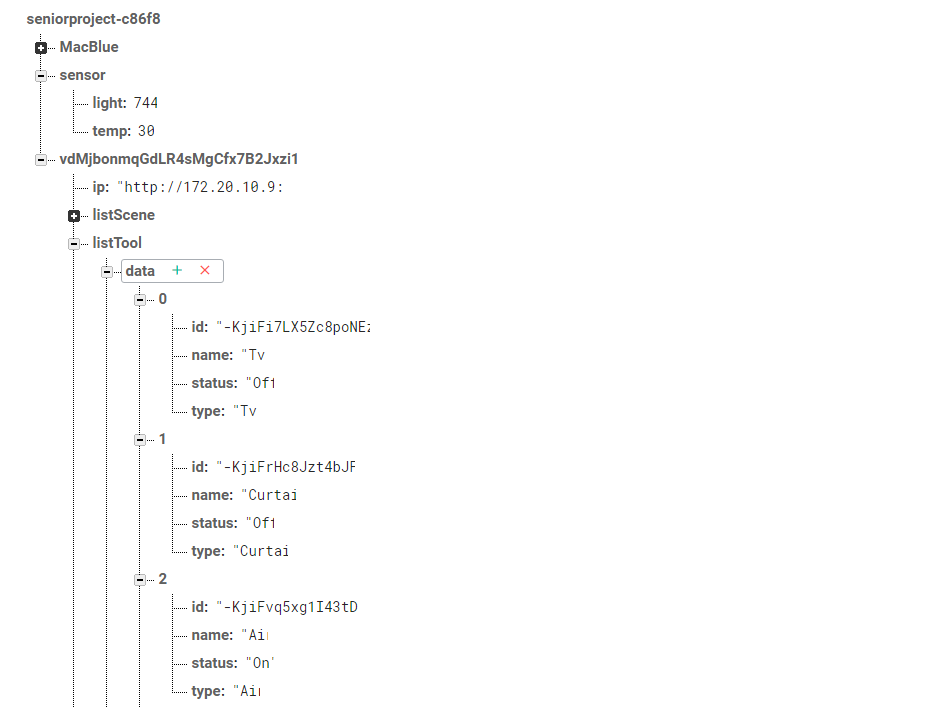
\includegraphics[width=1\textwidth]{firebase.png}
\caption{{\thi โครงสร้างข้อมูลของ} Firebase}
\label{firebase}
\end{figure}

	{\thi ซึ่งการที่การอ่านข้อมูลหรือการเขียนข้อมูลใน} firebase {\thi จะต้องทำข้อมูลให้เป็นฟอร์แมตใดก็ได้} {\thi โดยในการเขียนการอ่านจะต้องใช้ฟอร์แมตเดียวกันเท่านั้นซึ่งในโครงงานนี้จะใช้ฟอร์แมตเจสันที่สามารถอ่านเข้าใจได้ง่าย}

\section{Raspberry Pi}
	{\thi จากภาพ} 2.2 {\thi เป็นบอร์ดคอมพิวเตอร์ขนาดเล็กที่สามารถเชื่อมต่อกับจอมอนิเตอร์} {\thi คีย์บอร์ด} {\thi และเมาส์ได้} {\thi สามารถนำมาประยุกต์ใช้ในการทำโครงงานทางด้านอิเล็กทรอนิกส์} {\thi การเขียนโปรแกรม} {\thi หรือเป็นเครื่องคอมพิวเตอร์ตั้งโต๊ะขนาดเล็ก} {\thi ไม่ว่าจะเป็นการทำงาน} Spreadsheet Word Processing {\thi ท่องอินเทอร์เน็ต} {\thi ส่งอีเมลล์} {\thi หรือเล่นเกมส์} {\thi อีกทั้งยังสามารถเล่นไฟล์วีดีโอความละเอียดสูง} (High-Definition) {\thi ได้อีกด้วย}
{\thi บอร์ด} Raspberry Pi {\thi รองรับระบบปฏิบัติการลินุกซ์} (Linux Operating System) {\thi ได้หลายระบบ} {\thi เช่น} Raspbian (Debian) Pidora (Fedora) {\thi และ} Arch Linux {\thi เป็นต้น} {\thi โดยติดตั้งบน} SD Card {\thi บอร์ด} Raspberry Pi {\thi นี้ถูกออกแบบมาให้มี} CPU GPU {\thi และ} RAM {\thi อยู่ภายในชิฟเดียวกัน} {\thi มีจุดเชื่อมต่อ} GPIO {\thi ให้ผู้ใช้สามารถนำไปใช้ร่วมกับอุปกรณ์อิเล็กทรอนิกส์อื่นๆ} {\thi ได้อีกด้วย}
{\thi คุณสมบัติที่สำคัญของ} Raspberry Pi 3 {\thi ได้แก่}

\begin{itemize}
\item{CPU: Quad-core 1.2 GHz ARM Cortex-A53 {\thi แบบ} 64 bits}
\item{GPU: Broadcom VideoCore IV @ 400 MHz}
\item{Memory {\thi ขนาด} 1 GB (LPDDR2-900 SDRAM)}
\item{{\thi หน่วยความจุแบบ} MicroSD}
\item{4 USB ports}
\item{1 Ethernet port}
\item{802.11n Wireless LAN}
\item{Bluetooth 4.0}
\item{{\thi รองรับ} HDMI/Composite {\thi ผ่านทาง} RCA Jack}
\item{GPIO 40 pins}
\end{itemize}
\begin{figure}[h]
\centering
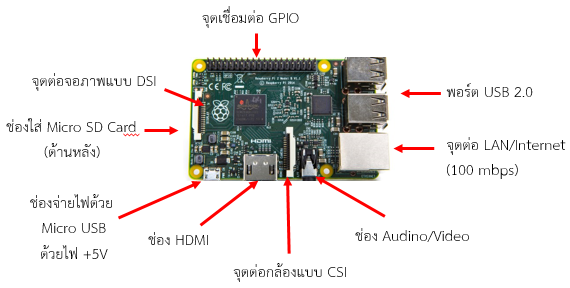
\includegraphics[width=0.8\textwidth]{raspberrypi.png}
\caption{Raspberry Pi}
\label{raspberrypi}
\end{figure}

\newpage
\section{Light Dependent Resistor}
{\thi เซ็นเซอร์แสง} (Optical Sensor) {\thi คืออุปกรณ์อิเล็กทรอนิกส์ที่เปลี่ยนแปลงค่าความต้านทาน} {\thi หรือการนำไฟฟ้า} {\thi ที่ไหลผ่านตัวมันได้} {\thi เมื่อมีแสงมาตกกระทบ} {\thi มีหลายชนิด}  {\thi ตัวต้านทานแปรค่าตามแสง} {\thi หรือ} LDR ({\thi ย่อมาจาก} Light Dependent Resistor) {\thi คืออุปกรณ์อิเล็กทรอนิกส์ที่ใช้ตรวจจับแสง} {\thi โดยหามีแสงมาตกกระทบน้อย} {\thi จะทำให้มีความต้านทานมาก} {\thi และหากมีแสงมาตกกระทบมาก} {\thi ความต้านทานจะน้อยลง}LDR {\thi นั้นทำมาจากสารกึงตัวนำแคดเมียมซัลไฟล์} (Cds) {\thi หรือแคดเมียมซีลิไนด์} (Cdse) {\thi นำมาฉาบลงบนแผ่นเซรามิคที่ใช้เป็นฐานรอง} {\thi ลักษณะตามภาพ} 2.3
\begin{figure}[h]
\centering
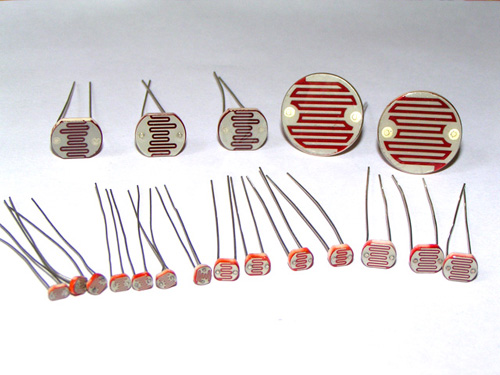
\includegraphics[width=0.6\textwidth]{LDR.jpg}
\caption{Light Dependent Resistor}
\label{LDR}
\end{figure}
\section{{\thi ไอซีเบอร์} DS1820}
DS18B20 {\thi เป็น} IC {\thi วัดอุณหภูมิแบบดิจิตอล} {\thi ของ} Dallas Semiconductor {\thi สามารถวัดอุณหภูมิเป็นหน่วยองศา} C {\thi ในช่วง} -55C {\thi ถึง} 125C {\thi ที่ความละเอียด} 9-12 {\thi บิต} {\thi และมีความแม่นยำอยู่ที่} 0.5C {\thi ในช่วง} -10C {\thi ถึง} 85C {\thi ในกรณีที่เป็นตัวถังแบบ} TO-92 {\thi นั้นจะมีโครงสร้าง} {\thi และขาดังแสดงในภาพที่} 1

{\thi การสื่อสารและควบคุม} DS18B20 {\thi นั้นสามารถทำได้โดยใช้บัสข้อมูลแบบ} 1-wire {\thi ของ} Dallas Semiconductor {\thi ซึ่งใช้สายสัญญาณเพียงแค่เส้นเดียวเท่านั้น} {\thi ภายใน} DS18B20 {\thi แต่ละตัวมีโค๊ดประจำตัวขนาด} 64 {\thi บิต} {\thi ทำให้สามารถใช้งาน} DS18B20 {\thi หลายตัวทำงานบนบัสแบบ} 1 wire {\thi พร้อมกันได้} {\thi นอกจากนี้} DS18B20 {\thi ยังสามารถทำงานในโหมดพาราสิต} (Parasite Power Mode) {\thi ซึ่งเป็นการทำงานโดยไม่ใช้ไฟเลี้ยง} {\thi แต่ใช้พลังงานจากสายสัญญาณ} 1-wire {\thi ซึ่งมีประโยชน์มากสำหรับการวัดอุณหภูมิระยะไกล} {\thi หรือในการใช้งานในที่} {\thi ๆ} {\thi มีเนื้อที่จำกัด} {\thi แต่ในบทความนี้จะกล่าวถึงรายละเอียดการใช้งานขั้นพื้นฐานในโหมดธรรมดาเท่านั้น} {\thi ลักษณะตามภาพ} 2.4 
\begin{figure}[h]
\centering
\includegraphics[width=0.6\textwidth]{icds18202.gif}
\caption{{\thi ไอซีเบอร์} DS1820}
\label{icds1802}
\end{figure}
\section{{\thi รีเลย์} (Relay)}

{\thi เป็นอุปกรณ์ที่เปลี่ยนพลังงานไฟฟ้าให้เป็นพลังงานแม่เหล็ก} {\thi เพื่อใช้ในการดึงดูดหน้าสัมผัสของ}(contact){\thi ให้เปลี่ยนสภาวะ} {\thi โดยการป้อนกระแสไฟฟ้าให้กับขดลวด} {\thi เพื่อทำการปิดหรือเปิดหน้าสัมผัสคล้ายกับสวิตช์อิเล็กทรอนิกส์} {\thi ซึ่งเราสามารถนำรีเลย์ไปประยุกต์ใช้} {\thi ในการควบคุมวงจรต่าง} {\thi ๆ} {\thi ในงานช่างอิเล็กทรอนิกส์มากมายรีเลย์} {\thi ลักษณะตามภาพ} 2.5 {\thi ประกอบด้วยส่วนสำคัญ} 2 {\thi ส่วนหลักก็คือ}
\begin{enumerate}
\item{{\thi ส่วนของขดลวด} (coil) {\thi เหนี่ยวนำกระแสต่ำ} {\thi ทำหน้าที่สร้างสนามแม่เหล็กไฟฟ้าให้แกนโลหะไปกระทุ้งให้หน้าสัมผัสต่อกัน} {\thi ทำงานโดยการรับแรงดันจากภายนอกต่อคร่อมที่ขดลวดเหนี่ยวนำนี้} {\thi เมื่อขดลวดได้รับแรงดัน}({\thi ค่าแรงดันที่รีเลย์ต้องการขึ้นกับชนิดและรุ่นตามที่ผู้ผลิตกำหนด}) {\thi จะเกิดสนามแม่เหล็กไฟฟ้าทำให้แกนโลหะด้านในไปกระทุ้งให้แผ่นหน้าสัมผัสต่อกัน}}
\item{{\thi ส่วนของหน้าสัมผัส} (contact) {\thi ทำหน้าที่เหมือนสวิตช์จ่ายกระแสไฟให้กับอุปกรณ์ที่เราต้องการนั่นเอง}}
\end{enumerate}
\begin{figure}[h]
\centering
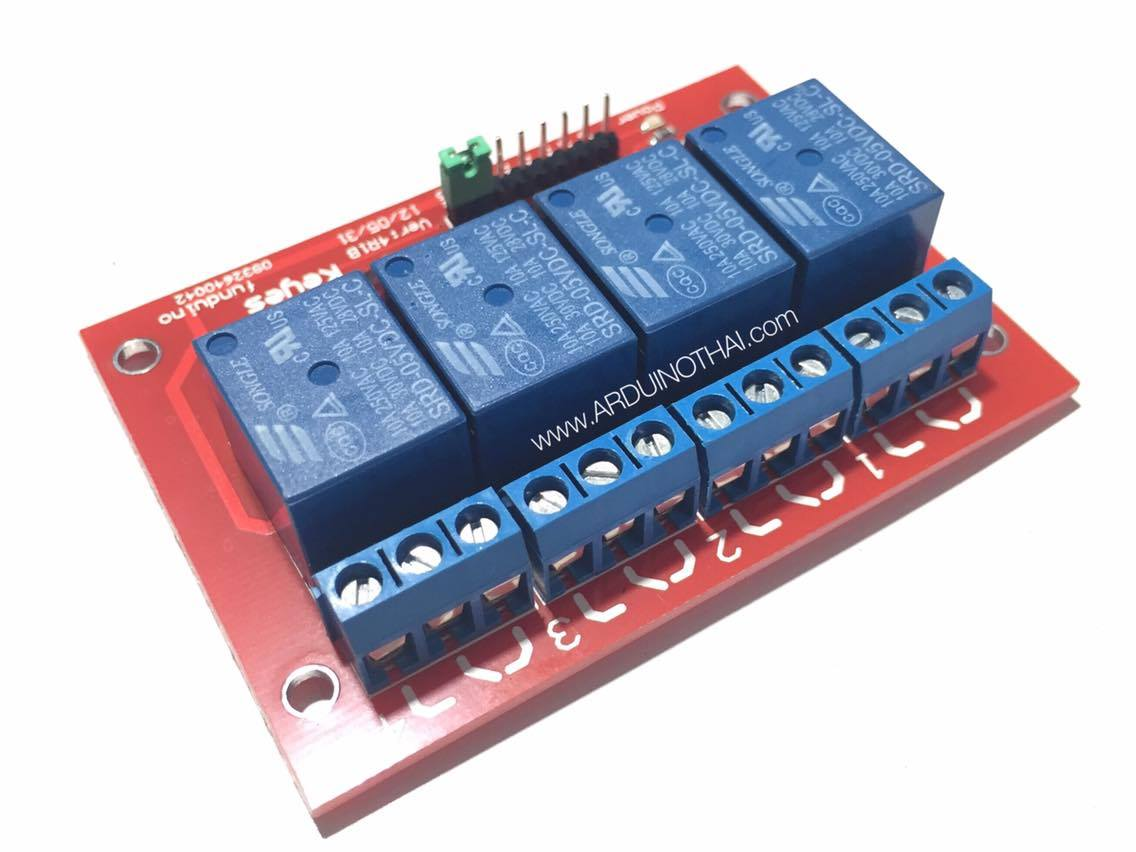
\includegraphics[width=0.6\textwidth]{relay.jpg}
\caption{{\thi รีเลย์} (Relay)}
\label{relay}
\end{figure}
\textbf{{\thi จุดต่อใช้งานมาตรฐาน} {\thi ประกอบด้วย}} ({\thi ตามภาพที่} 2.6)
\begin{enumerate}
\item{{\thi จุดต่อ} NC {\thi ย่อมาจาก} normal close {\thi หมายความว่าปกติดปิด} {\thi หรือ} {\thi หากยังไม่จ่ายไฟให้ขดลวดเหนี่ยวนำหน้าสัมผัสจะติดกัน} {\thi โดยทั่วไปเรามักต่อจุดนี้เข้ากับอุปกรณ์หรือเครื่องใช้ไฟฟ้าที่ต้องการให้ทำงานตลอดเวลาเช่น}}

\item{{\thi จุดต่อ} NO {\thi ย่อมาจาก} normal open {\thi หมายความว่าปกติเปิด} {\thi หรือหากยังไม่จ่ายไฟให้ขดลวดเหนี่ยวนำหน้าสัมผัสจะไม่ติดกัน} {\thi โดยทั่วไปเรามักต่อจุดนี้เข้ากับอุปกรณ์หรือเครื่องใช้ไฟฟ้าที่ต้องการควบคุมการเปิดปิดเช่นโคมไฟสนามหรือหน้าบ้าน}}

\item{{\thi จุดต่อ} C {\thi ย่อมากจาก} common {\thi คือจุดร่วมที่ต่อมาจากแหล่งจ่ายไฟ}}
\end{enumerate}
\begin{figure}[h]
\centering
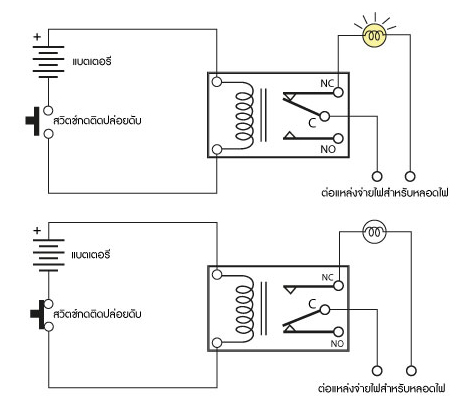
\includegraphics[width=0.6\textwidth]{relayCircuit.jpg}
\caption{Relay Circuit}
\label{relayCircuit}
\end{figure}

\section{Arduino}
Arduino {\thi เป็นบอร์ดไมโครคอนโทรเลอร์ตระกูล} AVR {\thi ที่มีการพัฒนาแบบ} Open Source{\thi คือมีการเปิดเผยข้อมูลทั้งด้าน} Hardware {\thi และ} Software {\thi ตัว} {\thi บอร์ด} Arduino {\thi ถูกออกแบบมาให้ใช้งานได้ง่าย} {\thi ดังนั้นจึงเหมาะสำหรับผู้เริ่มต้นศึกษา} {\thi ทั้งนี้ผู้ใช้งานยังสามารถดัดแปลง} {\thi เพิ่มเติม} {\thi พัฒนาต่อยอดทั้งตัวบอร์ด} {\thi หรือโปรแกรมต่อได้อีกด้วย}

{\thi ความง่ายของบอร์ด} Arduino {\thi ในการต่ออุปกรณ์เสริมต่างๆ} {\thi คือผู้ใช้งานสามารถต่อวงจรอิเล็กทรอนิคส์จากภายนอกแล้วเชื่อมต่อเข้ามาที่ขา} I/O {\thi ของบอร์ด} ({\thi ดูตัวอย่างภาพที่} 2.7) {\thi หรือเพื่อความสะดวกสามารถเลือกต่อกับบอร์ดเสริม} (Arduino Shield) {\thi ประเภทต่างๆ}({\thi ดูตัวอย่างภาพที่} 2.8){\thi เช่น} Arduino XBee Shield, Arduino Music Shield, Arduino Relay Shield, Arduino Wireless Shield, Arduino GPRS Shield {\thi เป็นต้น} {\thi มาเสียบกับบอร์ดบนบอร์ด} Arduino {\thi แล้วเขียนโปรแกรมพัฒนาต่อได้เลย}

\begin{figure}[h]
\centering
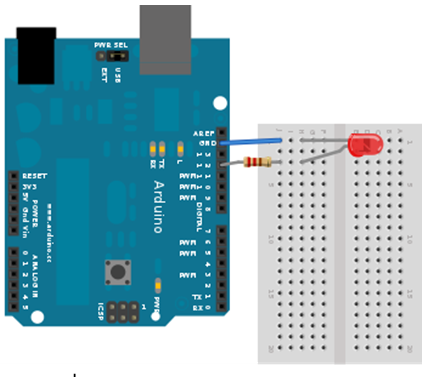
\includegraphics[width=0.5\textwidth]{arduino1.png}
\caption{Anduino + LED}
\label{android1}
\end{figure}
\begin{figure}[h]
\centering
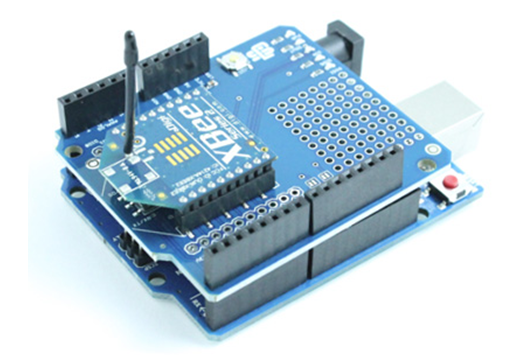
\includegraphics[width=0.5\textwidth]{arduino2.png}
\caption{Anduino + XBee}
\label{android2}
\end{figure}

\newpage
\section{NRF24L01}
{\thi โมดูล} NRF24L01 {\thi เป็นโมดูลสื่อสารไร้สาย} {\thi ที่สามารถเขียนโปรแกรมให้เป็นได้} {\thi ทั้งตัวรับและตัวส่ง} {\thi ตามภาพที่} 2.9 {\thi สามารถใช้กับ} Arduino {\thi ได้หลาย} {\thi ๆ} {\thi ตัวพร้อมกัน} {\thi มีความเร็ว} 2.4G {\thi จึงสื่อสารได้รวดเร็วและไม่ต้องการเสาอากาศที่ยาว} {\thi มีขนาดเล็กสะดวกในการต่อใช้งาน} {\thi สามารถประยุกต์ใช้งานได้หลายอย่างเช่น}  {\thi อุณหภูมิ} {\thi ความชื้น} {\thi การแจ้งเตือนต่าง} {\thi ๆ} {\thi ได้ในระยะ} 1-100 {\thi เมตร} {\thi โมดูลนี้ใช้ชิฟ}  nRF24L01+ m {\thi ทำงานด้วยความเร็วสูง} High-speed SPI interface {\thi ใช้พลังงานต่ำ} {\thi รองรับการทำงานร่วมกับ} Arduino 
\begin{figure}[h]
\centering
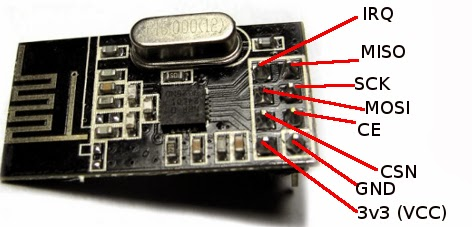
\includegraphics[width=0.4\textwidth]{sl.jpg}
\caption{NRF24L01}
\label{NRF24L01}
\end{figure}

\section{IR Transmitter}
	{\thi เป็นโมดูลที่ไว้ส่งสัญญาณอินฟาเรด} {\thi ตามภาพที่} 2.10 {\thi ที่ความยาวคลื่น} 940 {\thi นาโนเมตร}

\begin{figure}[h]
\centering
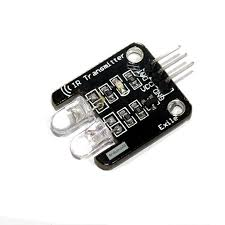
\includegraphics[width=0.29\textwidth]{irtransmitter.jpg}
\caption{IRTransmitter}
\label{IRTransmitter}
\end{figure}

\section{IR  Receiver}
	{\thi เป็นโมดูลที่ไว้รับสัญญาณอินฟาเรด} {\thi ตามภาพที่} 2.11
\begin{figure}[h]
\centering
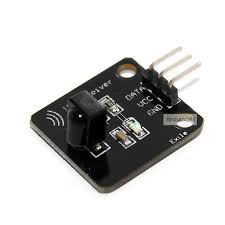
\includegraphics[width=0.29\textwidth]{irreceiver.jpg}
\caption{IR Receiver}
\label{IRReceiver}
\end{figure}

%%%%%%%%%%%%%%%%% {\thi การพัฒนา} %%%%%%%%%%%%%%%%%%%
\chapter{{\thi การพัฒนา}}


\section{{\thi อุปกรณ์}}
	\subsection{{\thi อุปกรณ์ด้านซอฟต์แวร์}}
		\begin{itemize}
			\item{{\thi คอมไพเลอร์ภาษา} Python {\thi ที่สนับสนุนภาษา} Python {\thi รุ่น} 3.5}
			\item{Python {\thi เป็นภาษาที่สร้างและพัฒนาใน} raspberry pi}
			\item{Python {\thi เป็นภาษาที่สร้างและพัฒนาใน} raspberry pi}
			\item{Node JS {\thi เป็น}  platform {\thi ที่สร้างและพัฒนาใน} IOS}
			\item{Flask {\thi เป็น} library {\thi ของ} python {\thi ที่ช่วยในการสร้างแล้วพัฒนา} web service}
			\item{Android studio {\thi ใช้เพื่อสร้างและพัฒนา} mobile application {\thi ในระบบ} Android}
			\item{Java {\thi เป็นภาษาที่ใช้สร้างและพัฒนา} mobile application {\thi ในระบบ} Android}
			\item{XML {\thi เป็นภาษาที่ใช้สร้าง} layout {\thi ของ} mobile application {\thi ในระบบ} Android}
			\item{ListView {\thi ใช้เพื่อแสดง} layout {\thi ให้เป็นแถว} {\thi ๆ} {\thi ที่เป็นแบบเดียวกัน} {\thi โดยใช้ข้อมูลที่เป็น} list}
			\item{Firebase realtime database {\thi ใช้สำหรับเก็บข้อมูลต่าง} {\thi ๆ} {\thi ของระบบ} {\thi และมีการ}   {\thi ตอบสนองเป็นแบบ} real time}
		\end{itemize}
\subsection{{\thi อุปกรณ์ด้านฮาร์ดแวร์}}

{\thi ในภาพ} 3.1 {\thi และ} 3.2 {\thi เป็นภาพวงจรของระบบซึ่งมี} raspberry pi {\thi เป็นส่วนกลางของระบบ} {\thi โดยคอยรับคำร้อง}(Request){\thi จากแอปพลิเคชันแล้วทำการส่งต่อไปยัง} Arduino {\thi เพื่อสั่งงานกับอุปกรณ์อื่น} {\thi ๆ} {\thi แบบไร้สายโดยผ่านโมดูล}(Module) NRF24L01
\begin{figure}[h]
\centering
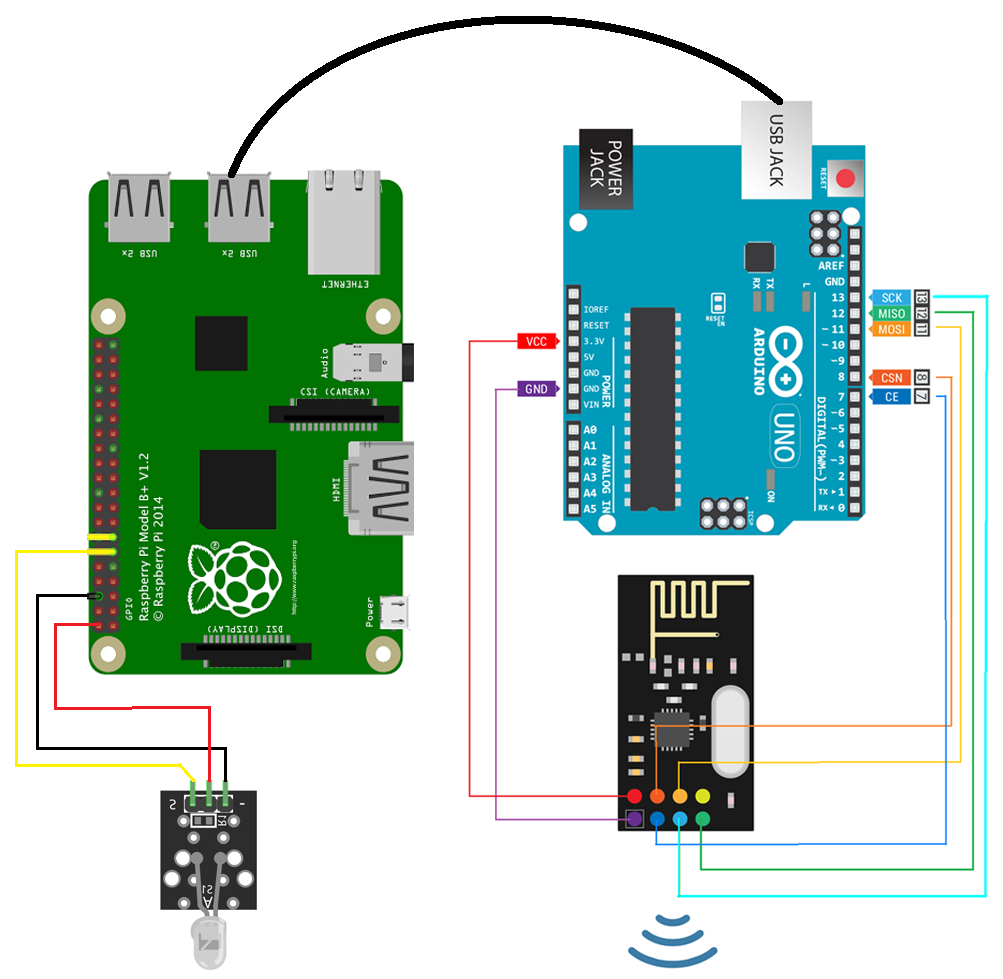
\includegraphics[width=0.9\textwidth]{cir1.png}
\caption{{\thi วงจงของระบบ}}
\label{cir2}
\end{figure}	
\begin{figure}[h]
\centering
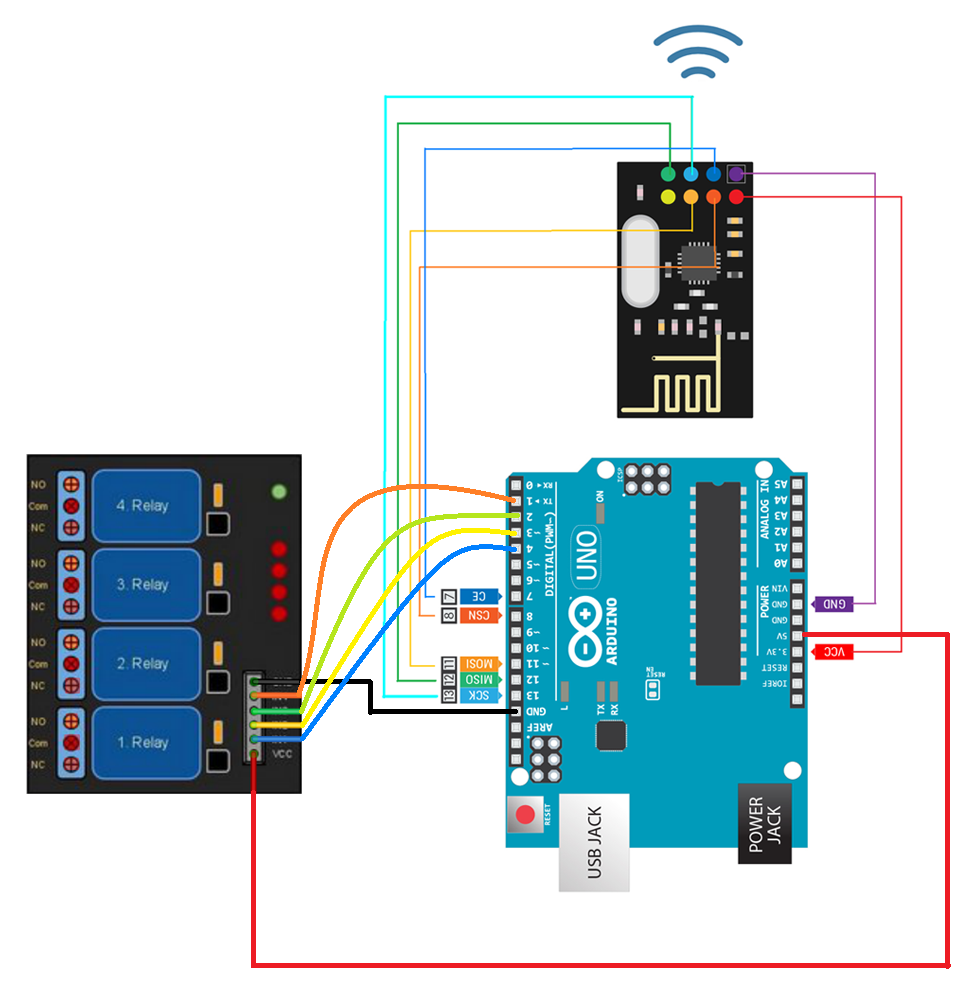
\includegraphics[width=0.9\textwidth]{cir2.png}
\caption{{\thi วงจงของระบบ}({\thi ต่อ})}
\label{cir2}
\end{figure}
\newpage
{\thi ในภาพ} 3.3 {\thi คือวงจรที่ใช้วัดอุณหภูมิเพื่อนำมาใช้ในระบบ} {\thi และ} {\thi ในภาพ} 3.4 {\thi คือวงจรที่ใช้วัดค่าความเข้มแสงเพื่อนำมาใช้ในระบบ}
\begin{figure}[h]
\centering
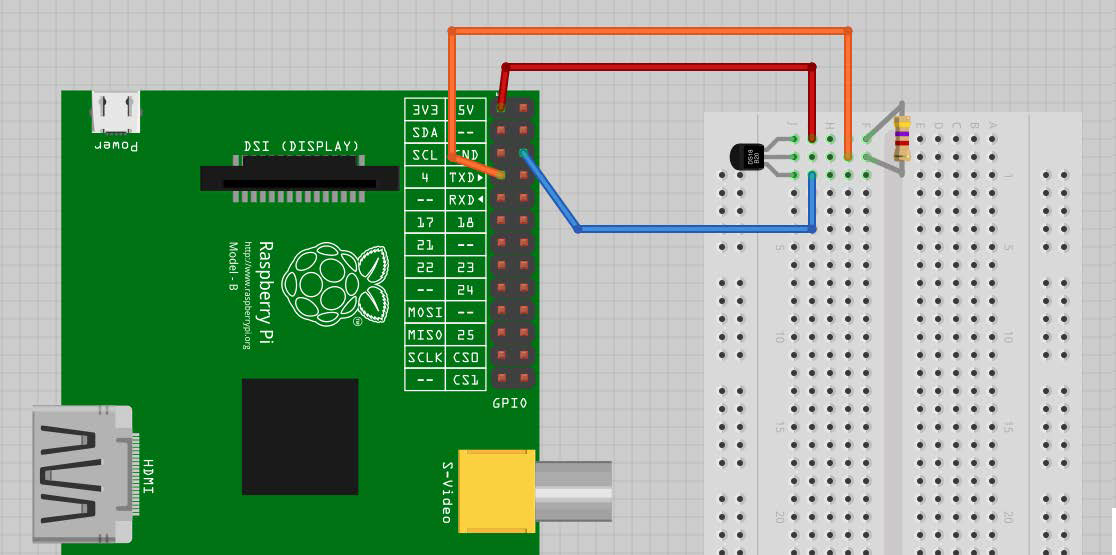
\includegraphics[width=0.5\textwidth]{tempSen.png}
\caption{{\thi วงจงของเซนเซอร์อุณหภูมิ}}
\label{cir2}
\end{figure}

\begin{figure}[h]
\centering
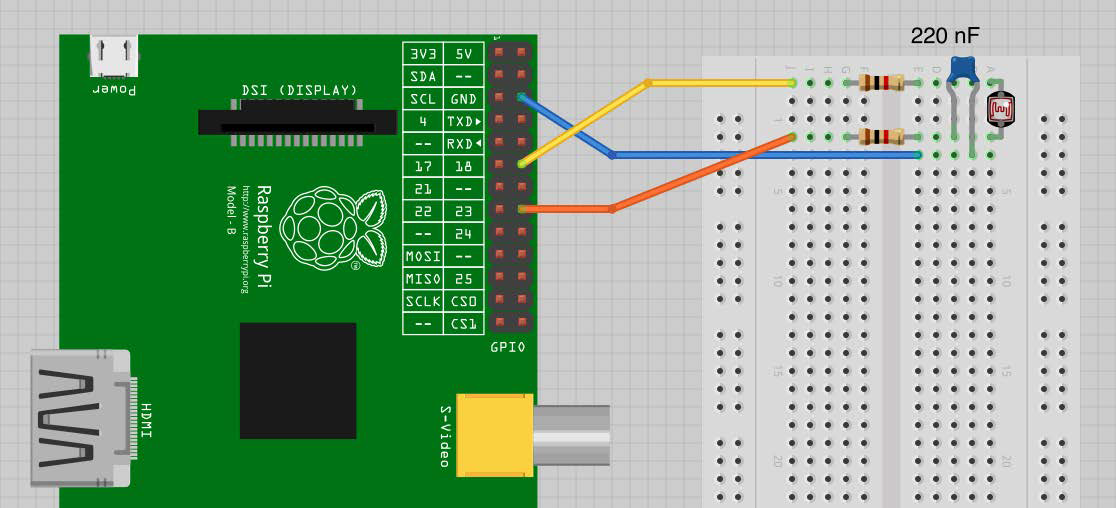
\includegraphics[width=0.5\textwidth]{lightSen.png}
\caption{{\thi วงจงของเซนเซอร์แสง}}
\label{cir2}
\end{figure}
\newpage	
\section{{\thi ภาพรวมของโครงงาน}}
	\subsection{{\thi รายละเอียดการทำงานของแอปพลิเคชัน}}
		{\thi ในภาพ} 3.13 {\thi เป็นภาพของโครงสร้างโดยรวมของระบบซึ่งจะแบ่งเป็น} 2 {\thi ส่วนดังนี้}
		\subsubsection{\textbf{{\thi ส่วนของ} Application}}

		{\thi แอปพลิเคชันจะอ่านข้อมูลจาก} Firebase({\thi สำหรับแอนดรอยด์}) {\thi และ} {\thi พื้นที่จัดเก็บข้อมูลของเครื่องโทรศัพท์}({\thi สำหรับไอโอเอส}){\thi ซึ่งจะมีข้อมูลอุปกรณ์และฉากที่สร้างไว้} {\thi โดยจะแสดงข้อมูลให้เห็นทางหนน้าต่างแอปพลิเคชันซึ่งจะแสดงอยู่ในรูปแบบอันดับ}(listview) {\thi สำหรับสั่งงานไปยังเว็บเซอร์วิส} 
	

	\subsubsection{\textbf{{\thi ส่วนของ} Server}}

	Raspberry PI {\thi จะทำหน้าที่เป็นเซิฟเวอร์ซึ่งเป็นเว็ปเซอร์วิสคอยรับรีเควสต่าง} {\thi ๆ} {\thi เข้ามาและประมวลผลคำสั่งแล้วสั่งการ} {\thi โมดูลต่าง} {\thi ๆ} {\thi โดยถ้าเป็นระบบปฏิบัติการแอนดรอยด์ส่งข้อมูลทางโปโตคอลเอชทีทีพี}(HTTP) {\thi ซึ่งจะทำการเช็คได้จาก} URL {\thi ที่ส่งมาแล้วสั่งการไปยัง} {\thi โมดูลที่ตั้งค่าไว้} {\thi ส่วนของระบบปฏิบัติการไอโอเอสจะทำการจำลองตัวเองให้} HomeKit{\thi สามารถเชื่อมต่อได้และส่งข้อมูลผ่านโปรโตคอล} HomeKit Acessory Protocol {\thi ซึ่ง} HomeKit {\thi จะทำการประมวลคำสั่งแล้วสั่งการไปยัง}Module{\thi ที่ตั้งค่าไว้เช่นกัน}

\subsubsection{\textbf{{\thi การทำงาน}}}

{\thi เมื่อมีคำสั่งแอปพลิเคชั่นจะส่งรีเควสไปหา} Raspberry PI {\thi ที่ทำหน้าที่เป็นเซอร์วิสซึ่งจะทำการประมวลผลคำสั่งที่ส่งมาแล้วก็จะทำงานตามที่ตั้งค่าไว้ซึ่งแต่ละคำสั่งจะเช่นเก็บ} {\thi ค่าไว้ใน} database {\thi เช่นถ้าสั่งปิดแอร์} Raspberry PI {\thi ก็จะส่งไปที่} IR transmitter {\thi ให้ทำหน้าที่ส่ง} {\thi สัญญาณอินฟาเรดไปที่แอร์โดยใช้} LIRC\cite{Ajtop}  {\thi หรือถ้าต้องการเช็คอุณหภูมิก็จะส่งไปหา}Temperature sensor\cite{Cookbook} {\thi เพื่อรับค่าอุณหภูมิมาแสดง}  {\thi ในแอปพลิเคชั่นนอกจากนี้ยังสามารถเช็คว่าผู้ใช้อยู่ใน} {\thi บ้านหรือไม่} {\thi ได้จากสัญญาณ}Bluetooth\cite{Bluetooth} {\thi จากโทรศัพท์อีกด้วยโดยในแอปพลิเคชั่นสามารถ} {\thi ตั้งค่าเป็นชุดคำสั่งต่าง} {\thi ๆ} {\thi ได้เอง} {\thi เช่น} {\thi เวลาออกเสียงว่า} {\thi “โหมดดูหนัง”} {\thi ให้เปิดแอร์}, {\thi เปิดทีวี} {\thi พร้อม} {\thi กับปิดม่านพร้อมกันได้หรือตั้งเงื่อนไขว่าถ้าอุณหภูมิมากกว่า} 37 {\thi องศาให้เปิดแอร์}
	
\begin{figure}[h]
\centering
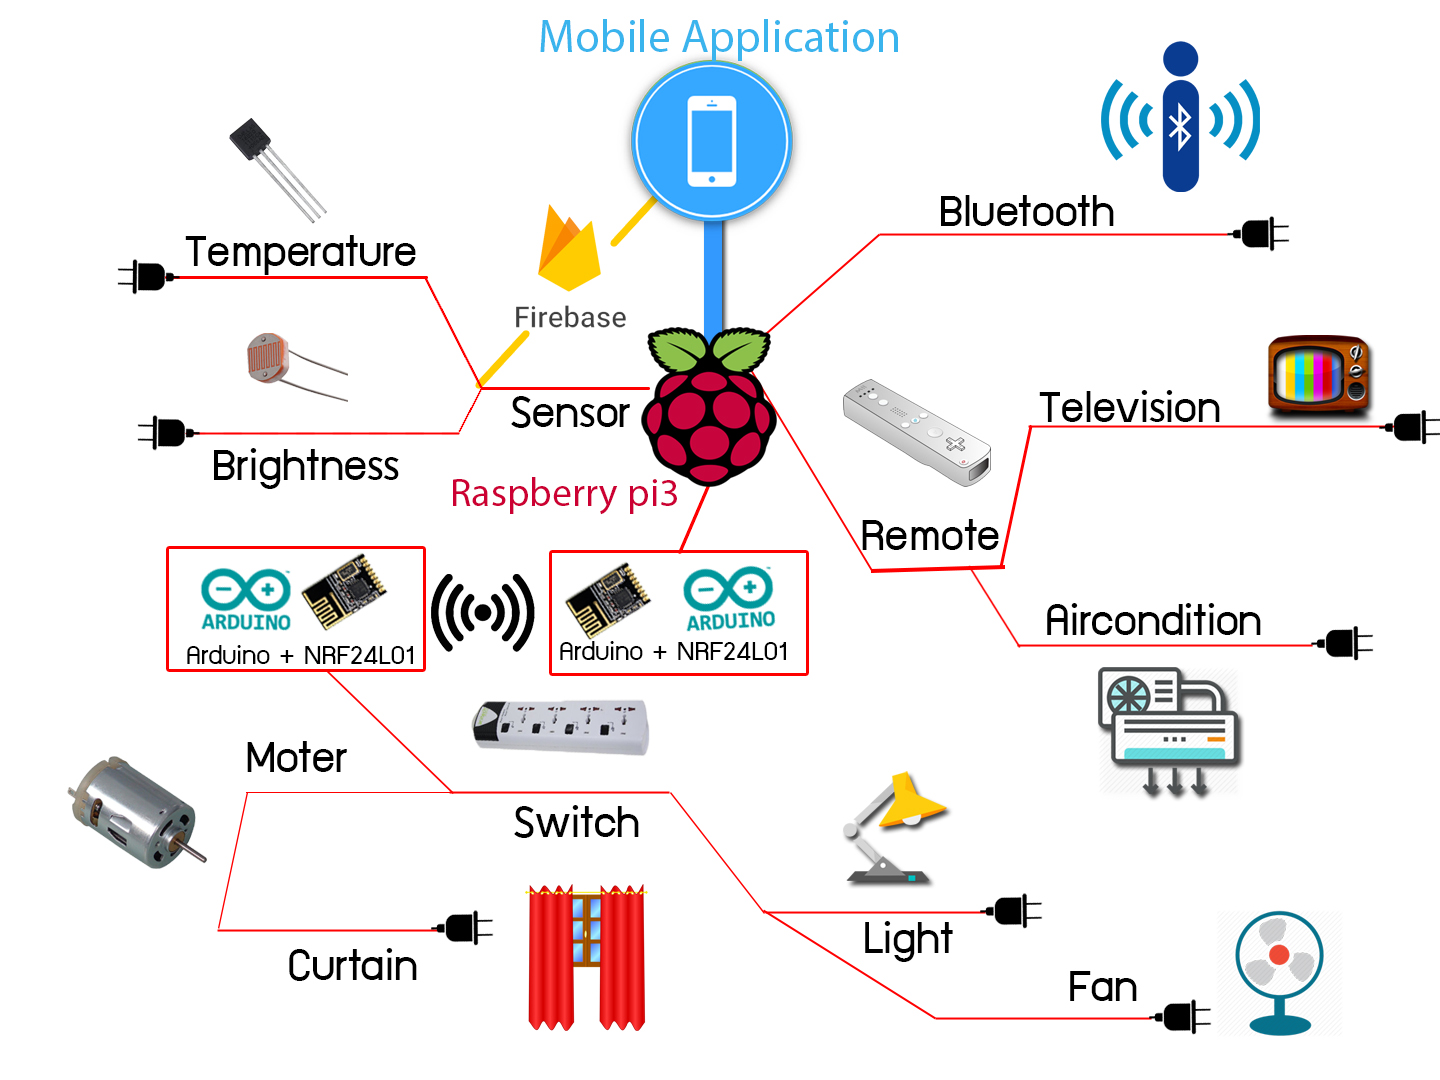
\includegraphics[width=1\textwidth]{simulat23.jpg}
\caption{{\thi โครงสร้างของระบบ}}
\label{simulat}
\end{figure}
	\subsection{{\thi โครงสร้างของฐานข้อมูล}}
	\begin{itemize}
		\item{System Table{\thi จากตาราง} 3.1 {\thi เป็นตารางที่ใช้เก็บข้อมูลของระบบ}}

		\item{User Table {\thi จากตาราง} 3.2 {\thi เป็นตารางที่ใช้เก็บข้อมูลผู้ใช้แต่ละคน}}

		\item{Tool Table {\thi จากตาราง} 3.3 {\thi เป็นตารางที่ใช้เก็บข้อมูลอุปกรณ์ของผู้ใช้งานนั้น} {\thi ๆ}}

		\item{Scene Table {\thi จากตาราง} 3.4 {\thi เป็นตารางที่ใช้เก็บข้อมูลฉากของผู้ใช้งานนั้น} {\thi ๆ}}
\end{itemize}

\begin{table}[h]
\centering
\caption{Syetem Table}
\label{and}\begin{tabular}{| c | c | c |}
\hline
Name         & Type   & Description           \\ \hline
system\_id   & int    & ID{\thi ของระบบ}             \\ \hline
mac\_blue    & string & {\thi เลข} MAC {\thi ของ} Bluetooth \\ \hline
status\_blue & bool   & {\thi สถานะของ} Bluetooth    \\ \hline
light        & double & {\thi ค่าความสว่างของระบบ}   \\ \hline
temp         & double & {\thi ค่าอุณหภูมิของระบบ}    \\ \hline
\end{tabular}
\end{table}

\begin{table}[h]
\centering
\caption{User Table}
\label{and}\begin{tabular}{| c | c | c |}
\hline
Name     & Type   & Description          \\ \hline
user\_id & string & ID {\thi ของผู้ใช้}         \\ \hline
ip       & string & IP {\thi ของ} server {\thi ที่ใช้} \\ \hline
tool     & Tool   & {\thi ข้อมูลของอุปกรณ์}     \\ \hline
\end{tabular}
\end{table}

\begin{table}[h]
\centering
\caption{Tool Table}
\label{and}\begin{tabular}{| c | c | c |}
\hline
Name     & Type   & Description     \\ \hline
tool\_id & string & ID {\thi ของอุปกรณ์}   \\ \hline
name     & string & {\thi ชื่อของอุปกรณ์}  \\ \hline
status   & bool   & {\thi สถานะของอุปกรณ์} \\ \hline
type     & string & {\thi ชนิดของอุปกรณ์}  \\ \hline
\end{tabular}
\end{table}

\begin{table}[h]
\centering
\caption{Scene Table}
\label{and}\begin{tabular}{| c | c | c |}
\hline
Name          & Type   & Description                    \\ \hline
scene\_id     & string & ID {\thi ของฉาก}                      \\ \hline
name          & string & {\thi ชื่อของอุปกรณ์}                 \\ \hline
ch\_bluetooth & bool   & {\thi สถานะของอุปกรณ์}                \\ \hline
bluetooth     & string & {\thi ชนิดของอุปกรณ์}                 \\ \hline
ch\_temp      & string & {\thi สถาน}option{\thi ของอุณหภูมิ}          \\ \hline
temp          & double & {\thi ค่าเงื่อนไขของ} option {\thi อุณหภูมิ} \\ \hline
ch\_light     & string & {\thi สถาน}option{\thi ของแสงสว่าง}          \\ \hline
light         & double & {\thi ค่าเงื่อนไขของ} option {\thi แสงสว่าง} \\ \hline
ch\_time      & string & {\thi สถานะของการตั้งเวลา}            \\ \hline
time          & string & {\thi เวลาที่ตั้ง}                    \\ \hline
\end{tabular}
\end{table}


















		

%%%%%%%%%%%%%%%%% {\thi ผลและวิจารณ์} %%%%%%%%%%%%%%%%%%%
\chapter{{\thi ผลและวิจารณ์}}


\section{{\thi การทดสอบ}}
	{\thi การทดสอบงานการใช้งานระบบควบคุมเครื่องใช้ไฟฟ้าภายในบ้านผ่านแอปพลิเคชันแบ่งการทดสอบออกเป็น} 2 {\thi ส่วน}  
	
\subsection{{\thi การทดสอบการทำงานแอปพลิเคชัน}}
{\thi การทดสอบเพื่อวัดผลการทำงานของแอปพลิเคชันโดยผู้พัฒนาระบบ} {\thi ซึ่งเป็นการทดสอบการทำงานขั้นพื้นฐานของระบบ} {\thi และขอบเขตการทำงานทั้งหมดของระบบประกอบไปด้วย} 2 {\thi ส่วนดังนี้}    
\subsubsection{{\thi ระบบปฎิบัติการไอโอเอส}}

{\thi ส่วนของแอปพลิเคชั่นควบคุม} {\thi วัดการทำงานแอปพลิเคชั่นควบคุม} {\thi ทดสอบ} {\thi โดยใช้โทรศัพท์มือถือ} iphone 6 plus  {\thi ระบบปฏิบัติการไอโอเอส} 10.3.1
{\thi ในภาพ} 4.1  {\thi เป็นหน้าเมนูของระบบไอโอเอสในหน้านี้จะแสดงลายละเอียดที่เราสามารถเลือกที่จะเพิ่มอุปกรณ์} {\thi สร้างคำสั่งด้วยเสียง} {\thi หรือแม้กระทั่งตั้งเวลาในการควบคุมอุปกรณ์ได้}
{\thi การเพิ่มอุปกรณ์ควบคุมนั้นทำได้โดยการกดที่ปุ่ม} Product  
\newpage
\begin{figure}[h]
\centering
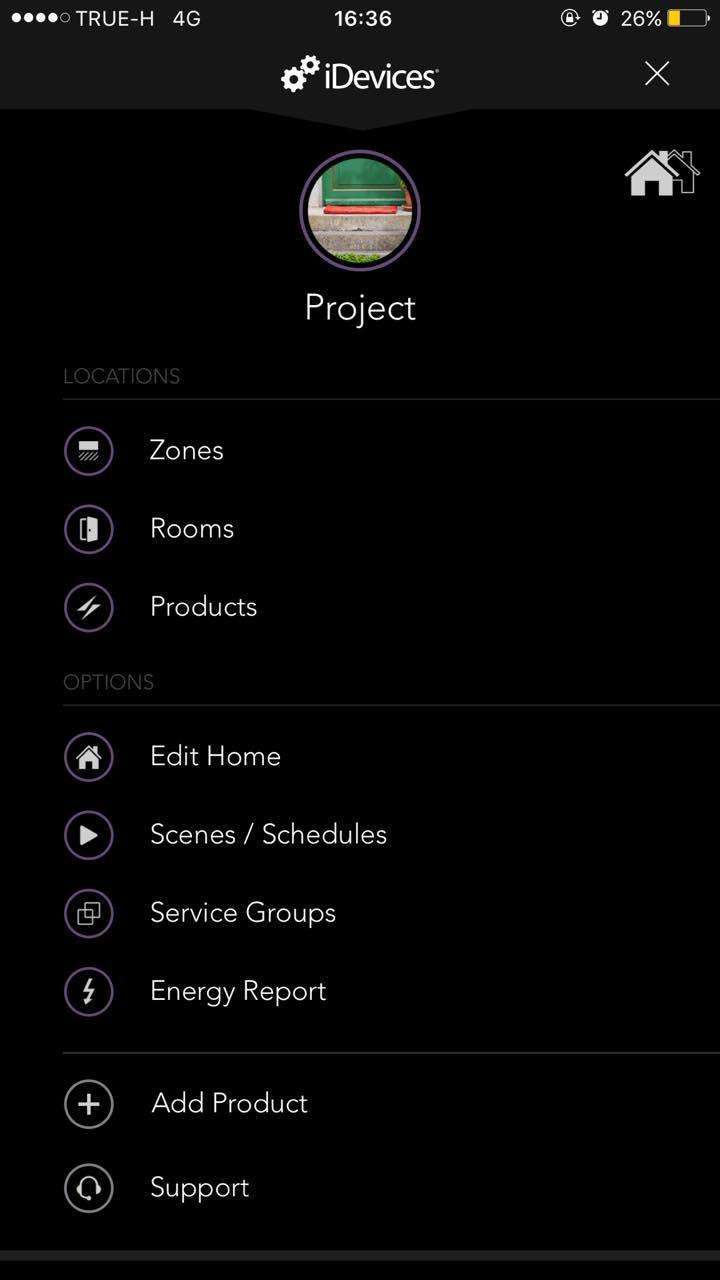
\includegraphics[width=0.27\textwidth]{1.jpg}
\caption{{\thi เมนูต่าง} {\thi ๆ} {\thi ของ} iDevices Homekit}
\label{ios1}
\end{figure}
{\thi แล้วจากนั้นจะปรากฏดังภาพ} 4.2 {\thi ก็สามารถกด} Add Product {\thi ได้เลย}
\begin{figure}[h]
\centering
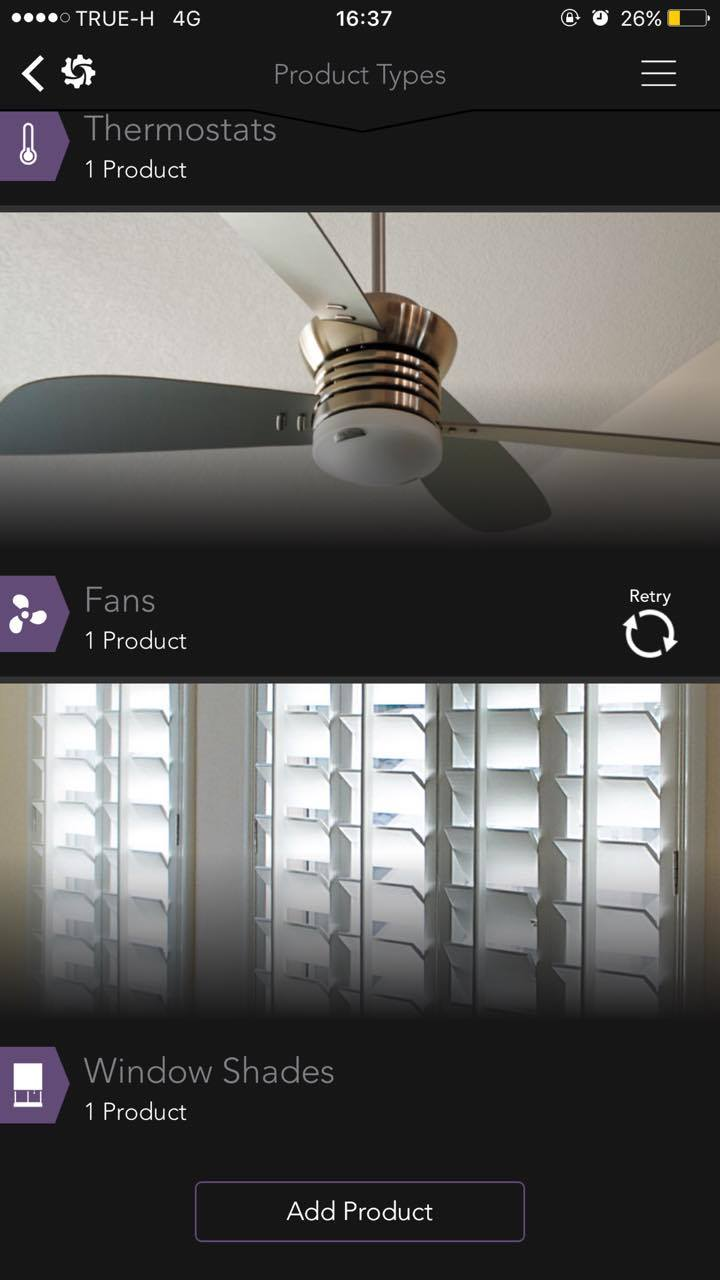
\includegraphics[width=0.27\textwidth]{2.jpg}
\caption{{\thi เพี่มอุปกรณ์ที่ต้องการเชื่อมต่อ}}
\label{ios2}
\end{figure}

{\thi ในการสร้างชุดคำสั่งด้วยเสียงนั้นสามารถทำได้โดยไปหน้าเมนูดังภาพ} 4.1 {\thi จากนั้นกด} Scenes {\thi จะปรากฏดังภาพ} 4.3    
\begin{figure}[h]
\centering
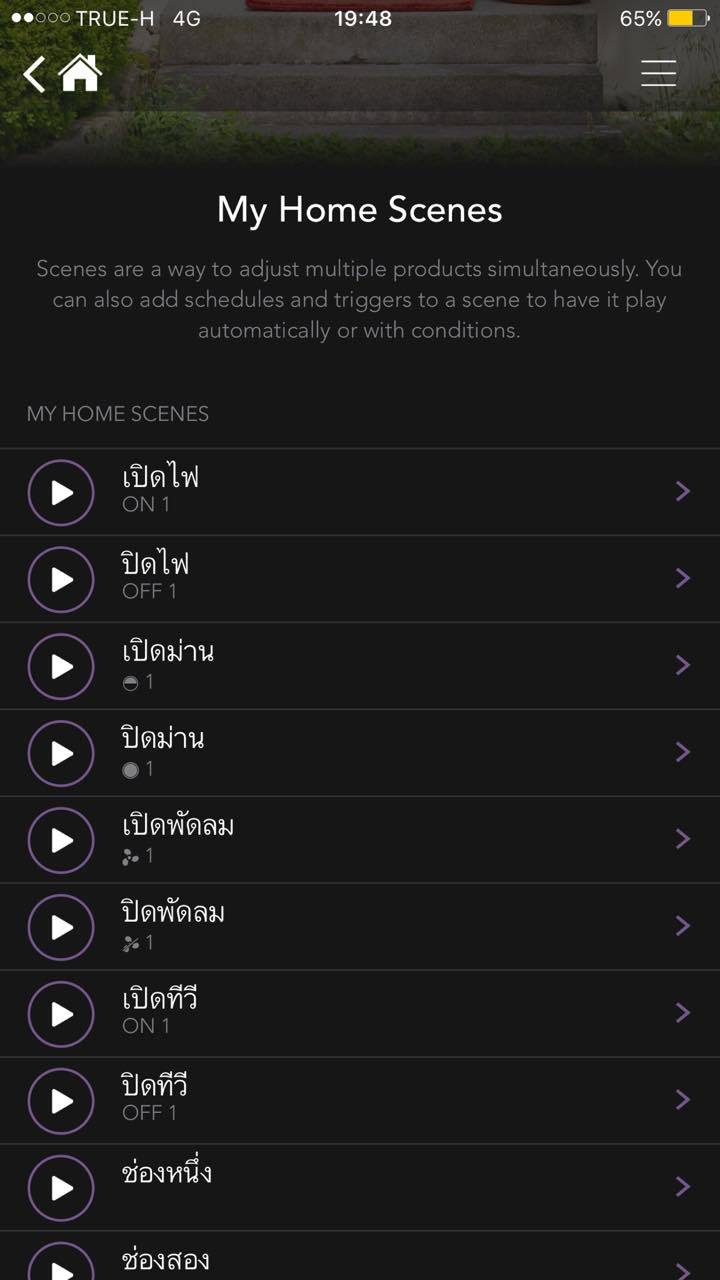
\includegraphics[width=0.27\textwidth]{6.jpg}
\caption{{\thi ชุดคำสั่งทั้งหมด}}
\label{ios6}
\end{figure}
\newpage
{\thi เลื่อนลงล่างสุดนั้นให้กด} Create New {\thi จะปรากฏดังภาพ} 4.4 {\thi ในหน้านี้เราสามารถเลือกอุปกรณ์ที่เราจะทำการสั่งการควบคุมได้เลย} {\thi สามารถเลือกได้มากกว่า} 1 {\thi อุปกรณ์} 
\begin{figure}[h]
\centering
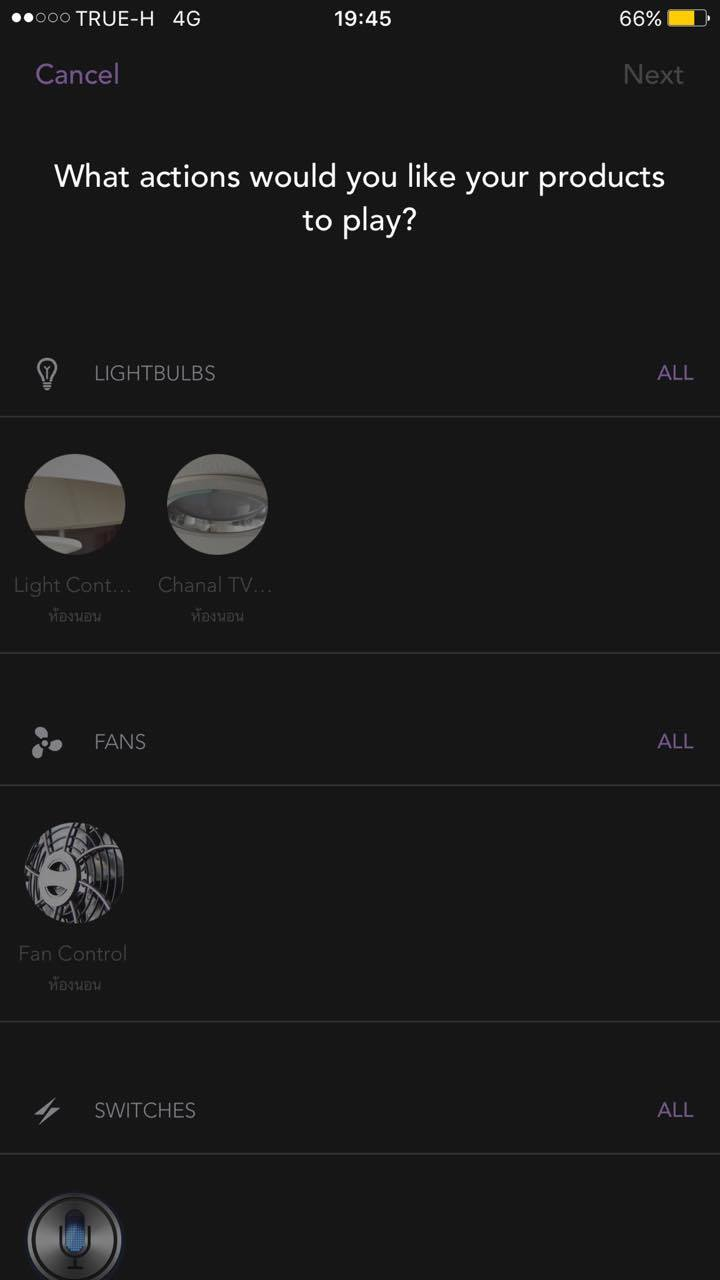
\includegraphics[width=0.27\textwidth]{4.jpg}
\caption{{\thi เลือกอุปกรณ์ในชุดคำสั่ง}}
\label{ios4}
\end{figure}

{\thi จากนั้นกด} Next {\thi จะปรากฏดังภาพ} 4.5 {\thi ในหน้านี้เป็นคำสั่งที่เราสามารถเลือกที่จะสั่งเสียงด้วยคำพูดต่าง} {\thi ๆ} 
\begin{figure}[h]
\centering
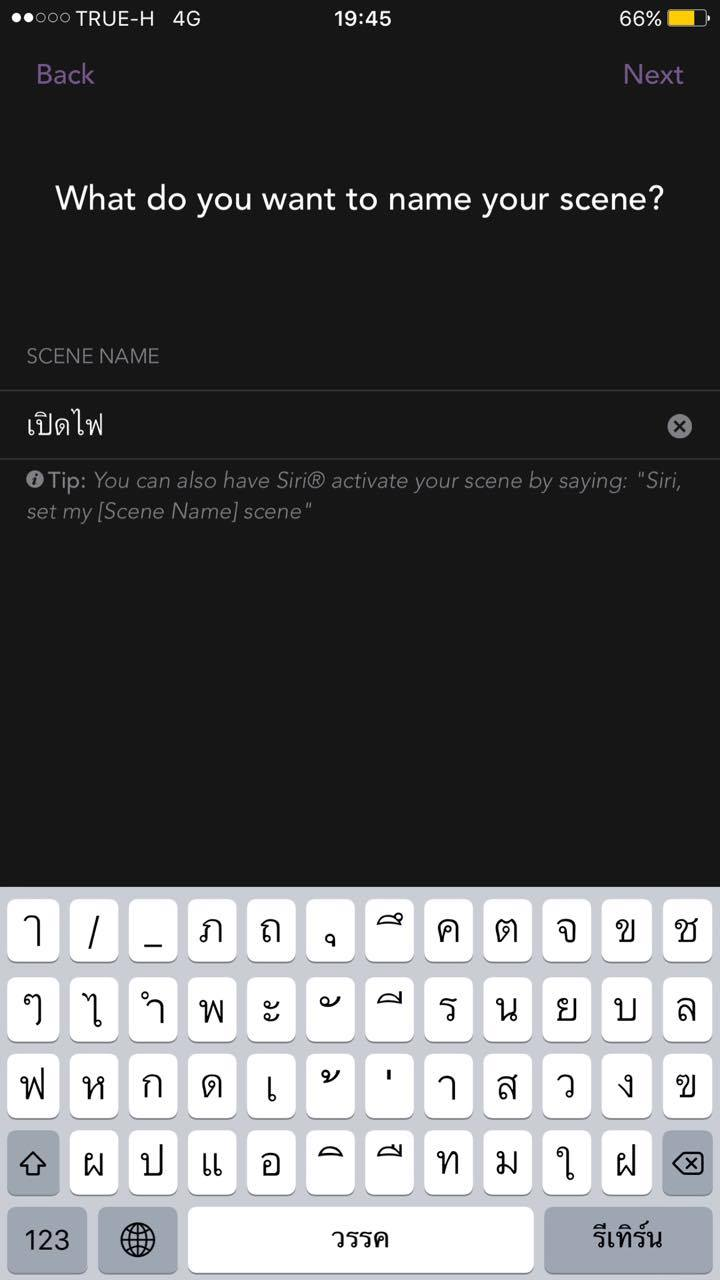
\includegraphics[width=0.27\textwidth]{5.jpg}
\caption{{\thi คำพูดที่ต้องการใช้ในการสั่งเสียง}}
\label{ios5}
\end{figure}
\newpage
{\thi ส่วนการตั้งเวลานั้นสามารถทำได้โดยไปที่หน้าเมนูดังภาพ} 4.1 {\thi จากนั้นกด} Schedules {\thi จะปรากฏดังภาพ} 4.6 
\begin{figure}[h]
\centering
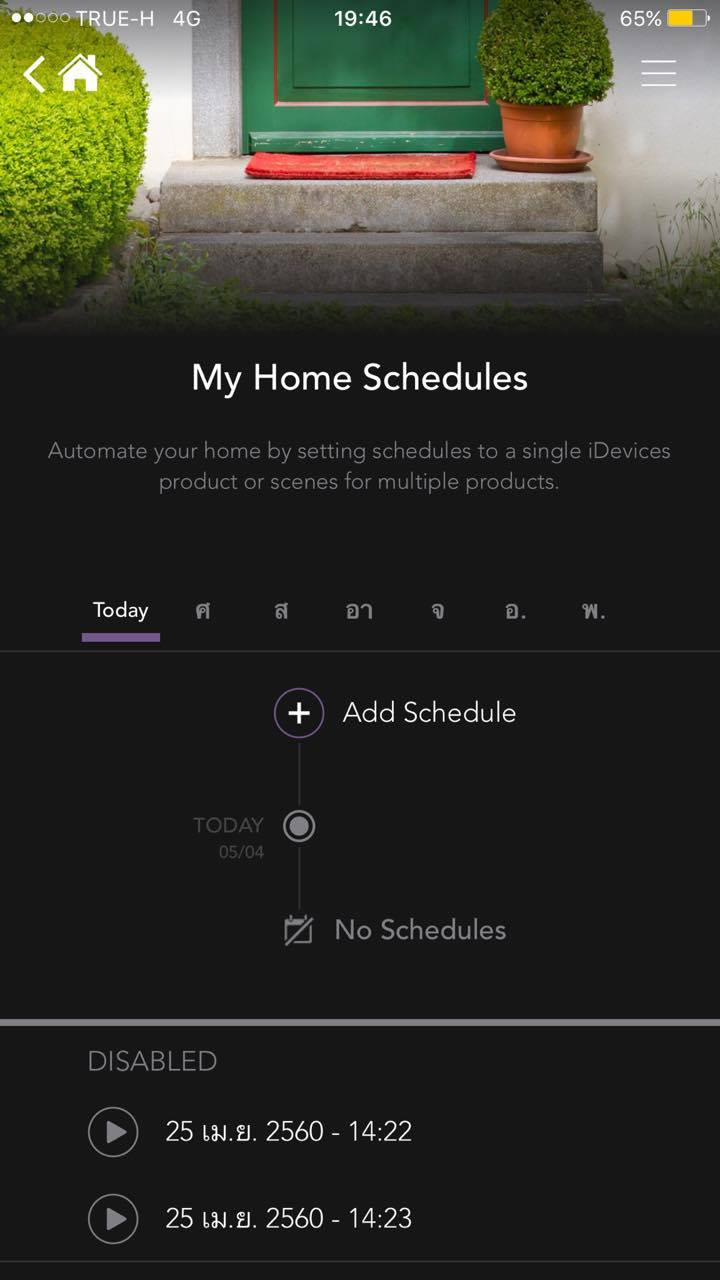
\includegraphics[width=0.27\textwidth]{7.jpg}
\caption{{\thi เพิ่มชุดคำสั่งลงใน}  Schedules}
\label{ios7}
\end{figure}
\newpage
{\thi กด} Add Schedules {\thi จะปรากฏดังภาพ} 4.7 {\thi ในหน้านี้จะให้เราเลือกว่าเราจะเอาชุดคำสั่งไหนบ้างที่จะทำการเพิ่มเข้าไปใน} Schedules  
\begin{figure}[h]
\centering
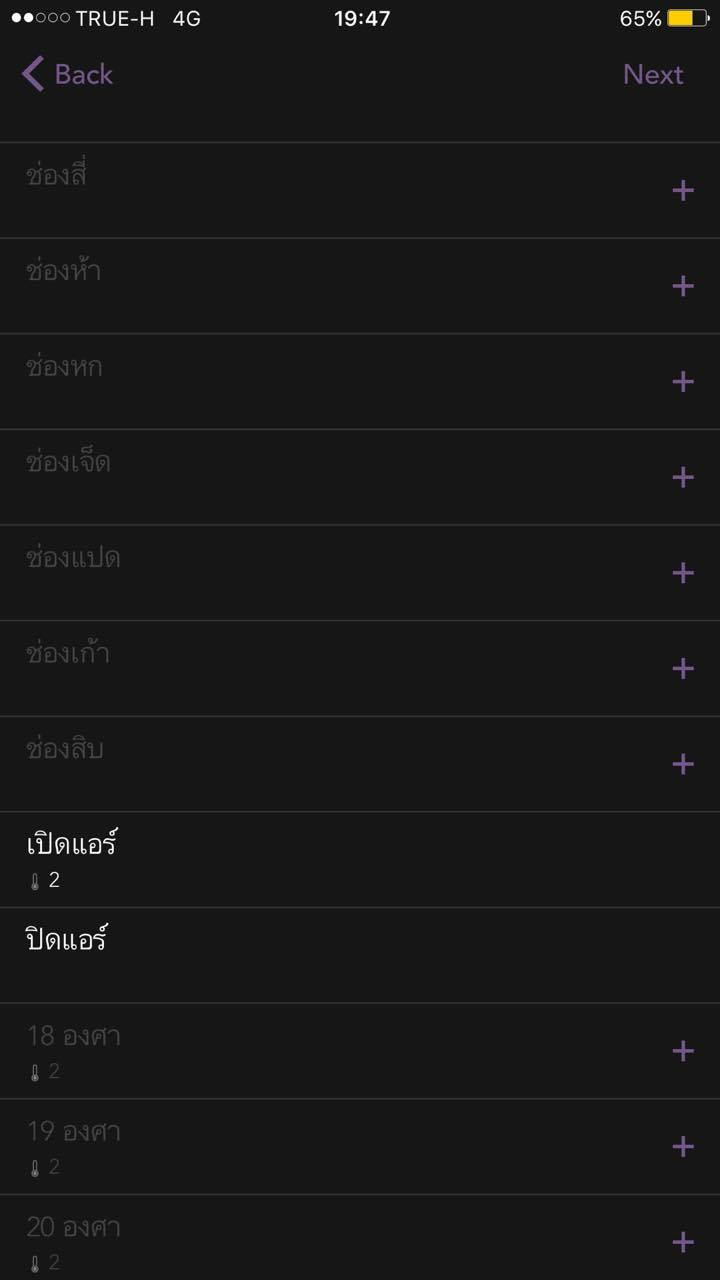
\includegraphics[width=0.27\textwidth]{8.jpg}
\caption{{\thi เลือกชุดคำสั่งที่ต้องการลงใน} Schedule}
\label{ios8}
\end{figure}

{\thi เมื่อเลือกเสร็จแล้วทำการกด} Next {\thi จะปรากฏดังภาพ} 4.8 {\thi ในหน้านี้เราสามารถทำการเลือกได้ว่าจะเอา} {\thi วัน}/{\thi เวลา} {\thi อะไร}
\begin{figure}[h]
\centering
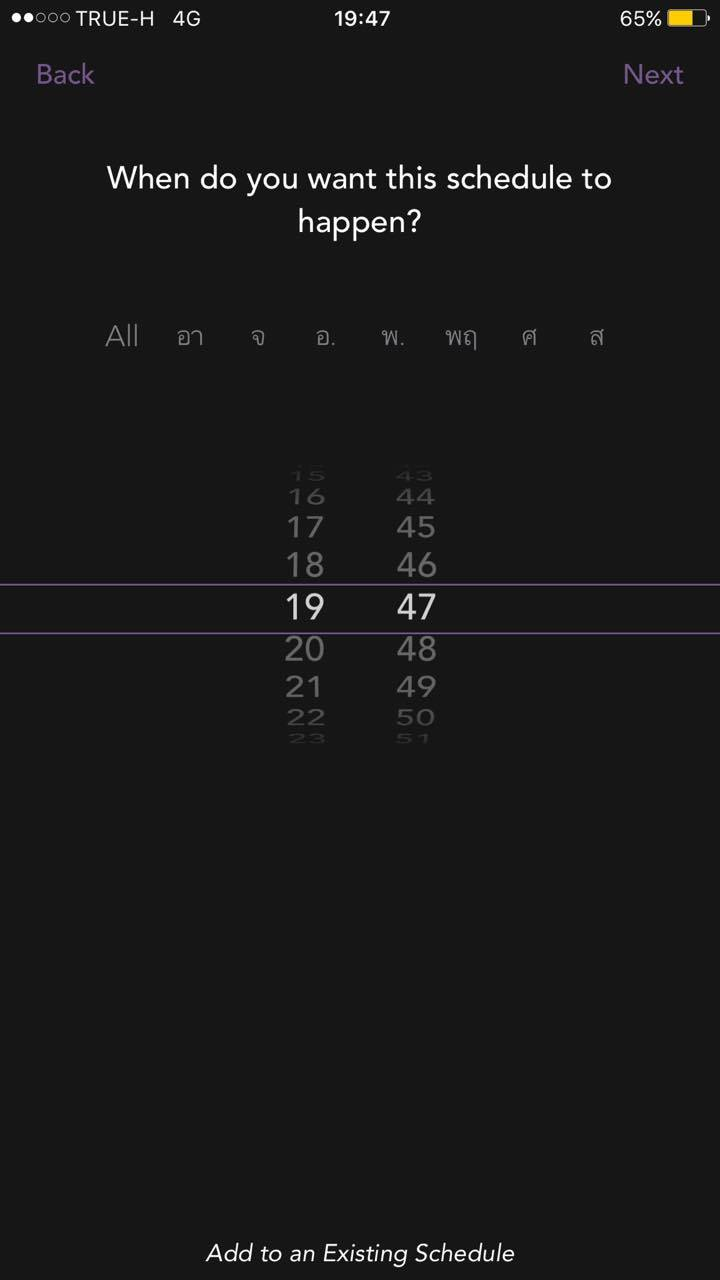
\includegraphics[width=0.27\textwidth]{9.jpg}
\caption{{\thi เลือก} {\thi วัน}/{\thi เวลา} {\thi ที่ต้องการลงใน} Schedule}
\label{ios9}
\end{figure}

\newpage
\subsubsection{{\thi ระบบปฎิบัติการ} Android}
{\thi ส่วนของแอปพลิเคชั่นควบคุม} {\thi วัดการทำงานแอปพลิเคชั่นควบคุม} {\thi ทดสอบ} {\thi โดยใช้โทรศัพท์มือถือ} Samsung {\thi ระบบปฏิบัติการ} Android 4.4.2  

{\thi ในภาพ} 4.9 {\thi เป็นหน้าแรกของ} {\thi แอปพลิเคชัน} {\thi ในระบบปฏิบัติการ} {\thi แอนดรอยด์} {\thi ซึ่งจะเป็นหน้าให้} {\thi ลงชื่อเข้าใช้โดยใช้} google account 
\begin{figure}[h]
\centering
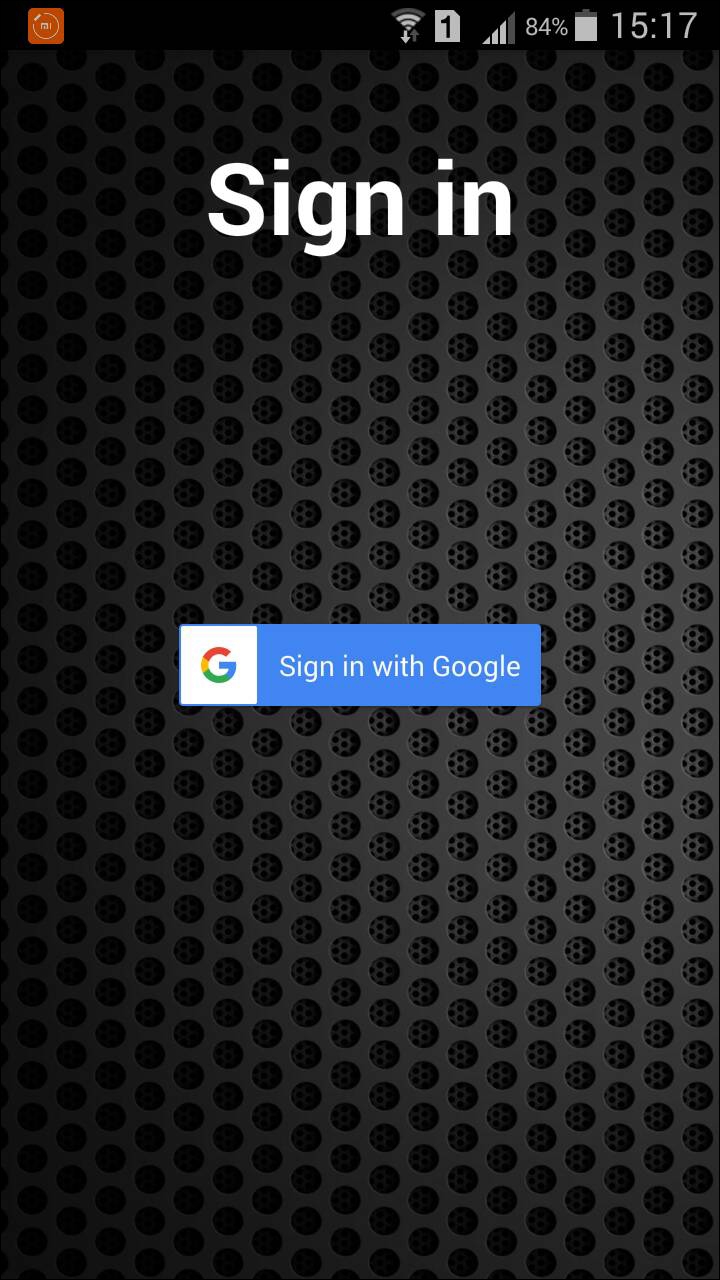
\includegraphics[width=0.27\textwidth]{login1.jpg}
\caption{sign in {\thi ด้วย} google account}
\label{login1}
\end{figure}

{\thi เมื่อกดปุ่มแล้วจะแสดงหน้าต่างขึ้นมาดังภาพ} 4.10 {\thi เพื่อให้เลือกหรือเพิ่ม} 

\begin{figure}[h]
\centering
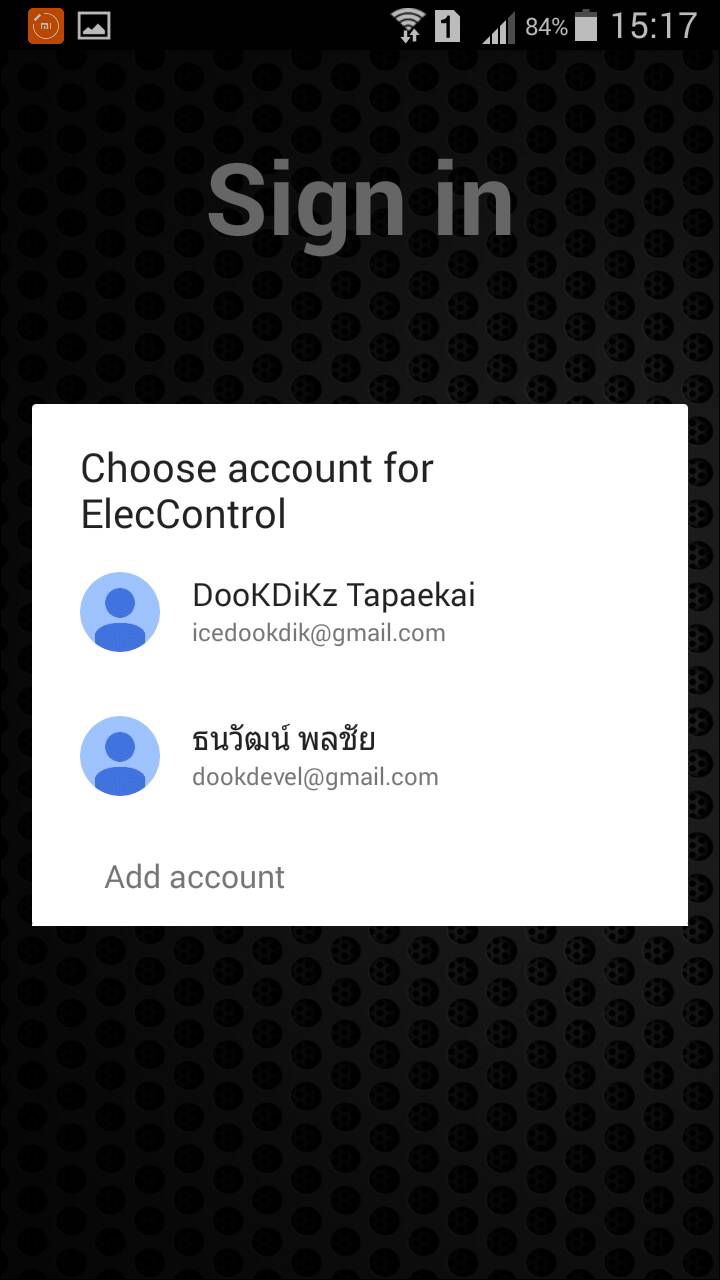
\includegraphics[width=0.27\textwidth]{login2.jpg}
\caption{{\thi เลือก} google account}
\label{login2}
\end{figure}
{\thi จากนั้นเมื่อทำการลงชื่อเข้าใช้} {\thi ไปแล้วจะเข้าสู่หน้าหลัก} {\thi ดังภาพที่} 4.11 {\thi ซึ่งจะมีหน้าต่างให้กรอก} IP address {\thi เพื่อเชื่อมต่อเว็ปเซอร์วิส} 
\newpage

\begin{figure}[h]
\centering
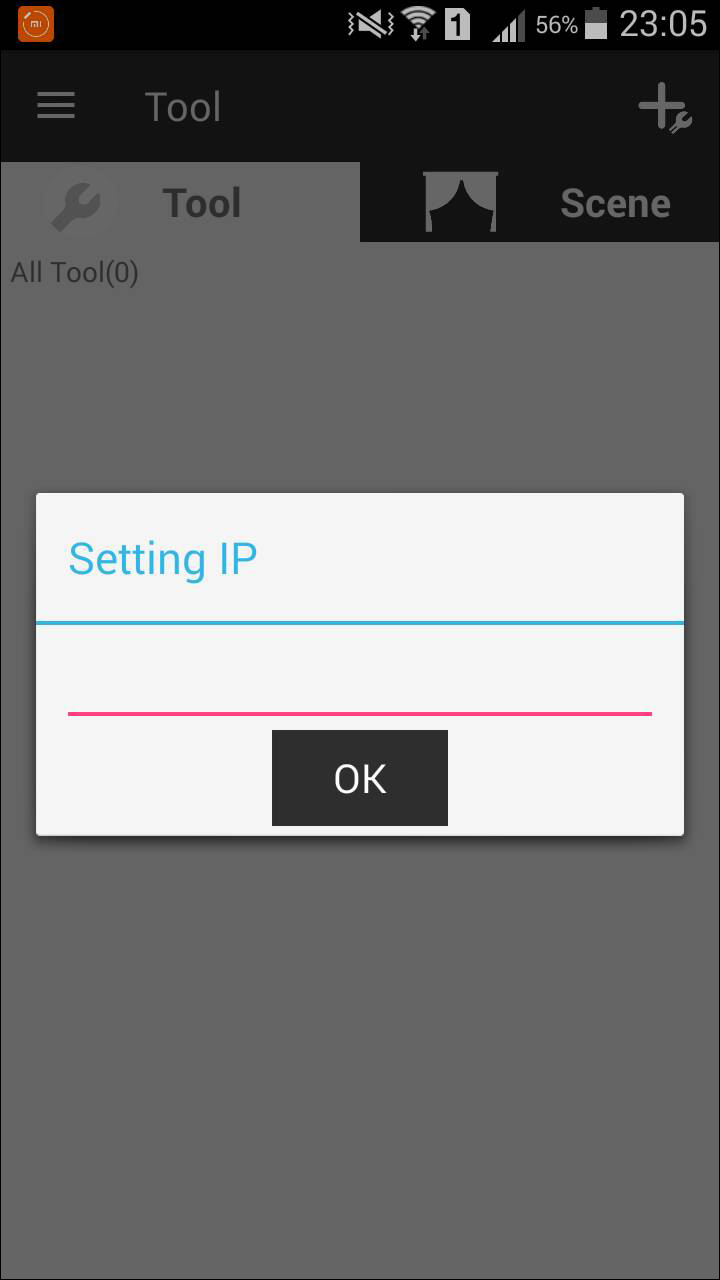
\includegraphics[width=0.27\textwidth]{setipstart.jpg}
\caption{{\thi ตั้งค่า} IP {\thi ของ} web service}
\label{setIPStart}
\end{figure}

{\thi เมื่อกรอกแล้วจะแสดงดังภาพ} 4.12 ({\thi ยังไม่ได้สร้าง}) {\thi คือหน้าที่จะแสดง} {\thi อุปกรณ์ไฟฟ้า}  {\thi และเมื่อกดไปที่} scene {\thi จะแสดงฉาก} {\thi ดังภาพ} 4.13 ({\thi ยังไม่ได้สร้าง})
\newpage
\begin{figure}[h]
\centering
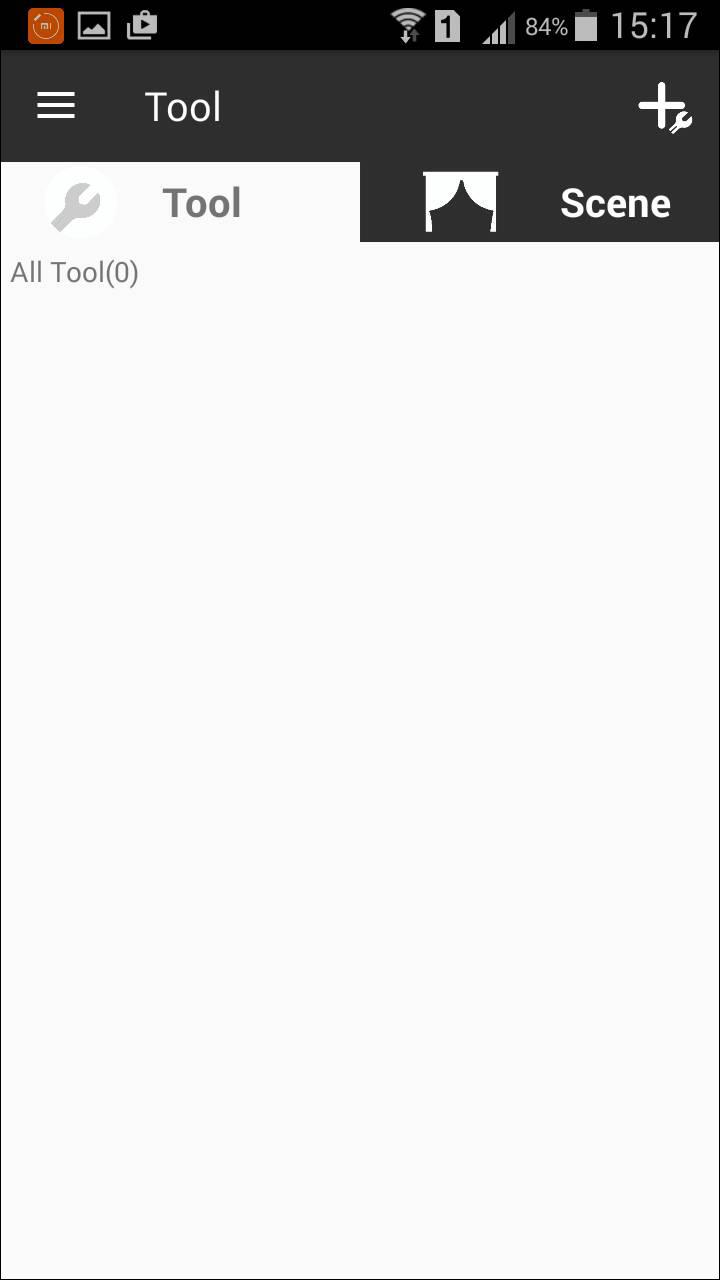
\includegraphics[width=0.27\textwidth]{toolpageempty.jpg}
\caption{tool page}
\label{toolpageempty}
\end{figure}

\begin{figure}[h]
\centering
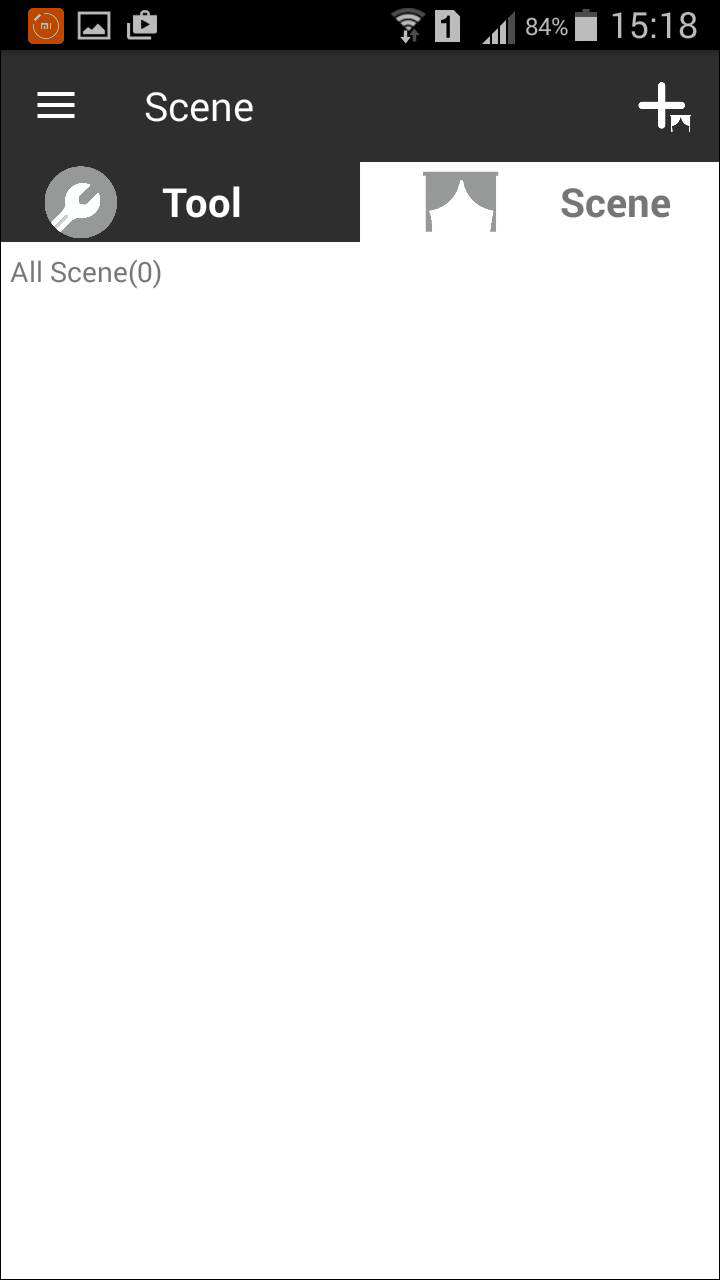
\includegraphics[width=0.27\textwidth]{scenepage.jpg}
\caption{Scene page}
\label{scenepage}
\end{figure}

{\thi ในภาพ} 4.14 {\thi จะเป็นเมนูซึ่งก็จะ} Add tool, Add Scene, Add Bluetooth Address, Set IP Address, Voice, Sign out {\thi และจะแสดง} {\thi อุณหภูมิ} {\thi และความเข้มของแสง}
\begin{figure}[h]
\centering
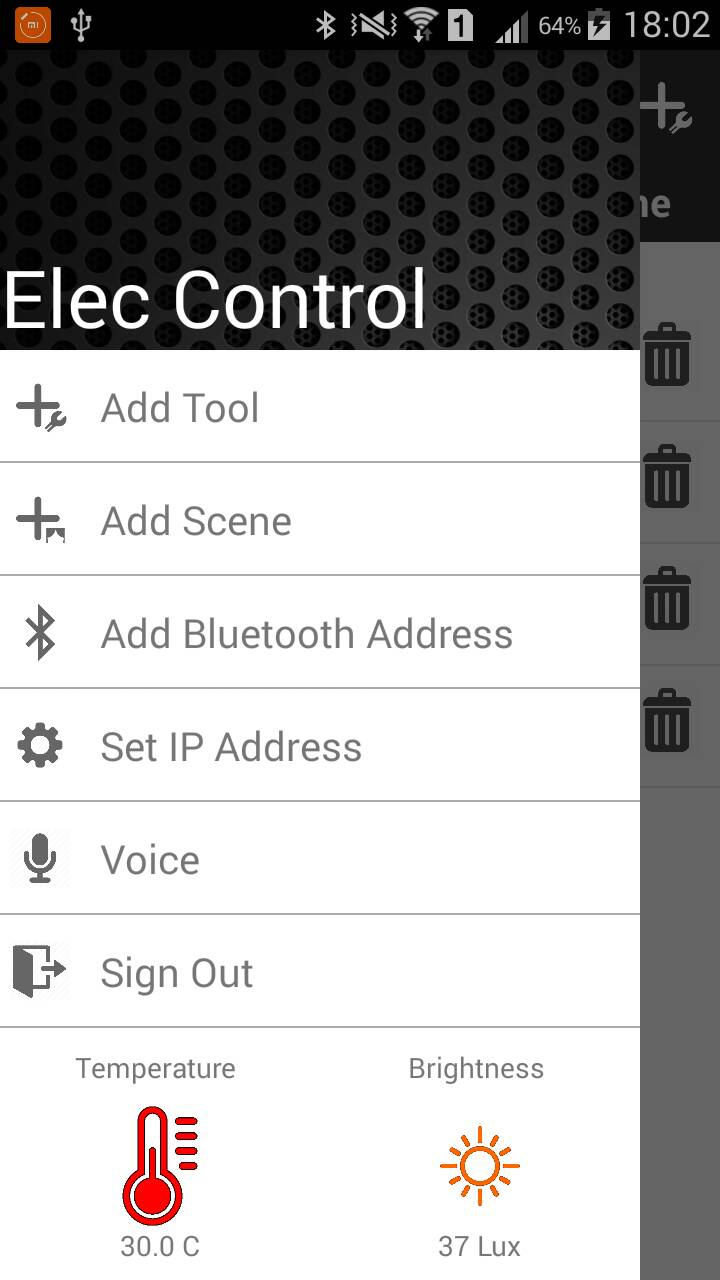
\includegraphics[width=0.27\textwidth]{hammenu.jpg}
\caption{menu}
\label{hammenu}
\end{figure}
\newpage
{\thi เมื่อกดเมนูเพิ่มอุปกรณ์}(Add tool) {\thi ก็จะแสดงดังภาพ} 4.15 {\thi ซึ่งจะมีให้เลือก} 3 {\thi รูปแบบ} {\thi คือ} {\thi รีโมต}, {\thi สวิตช์} {\thi และ} {\thi ผ้าม่าน}
\begin{figure}[h]
\centering
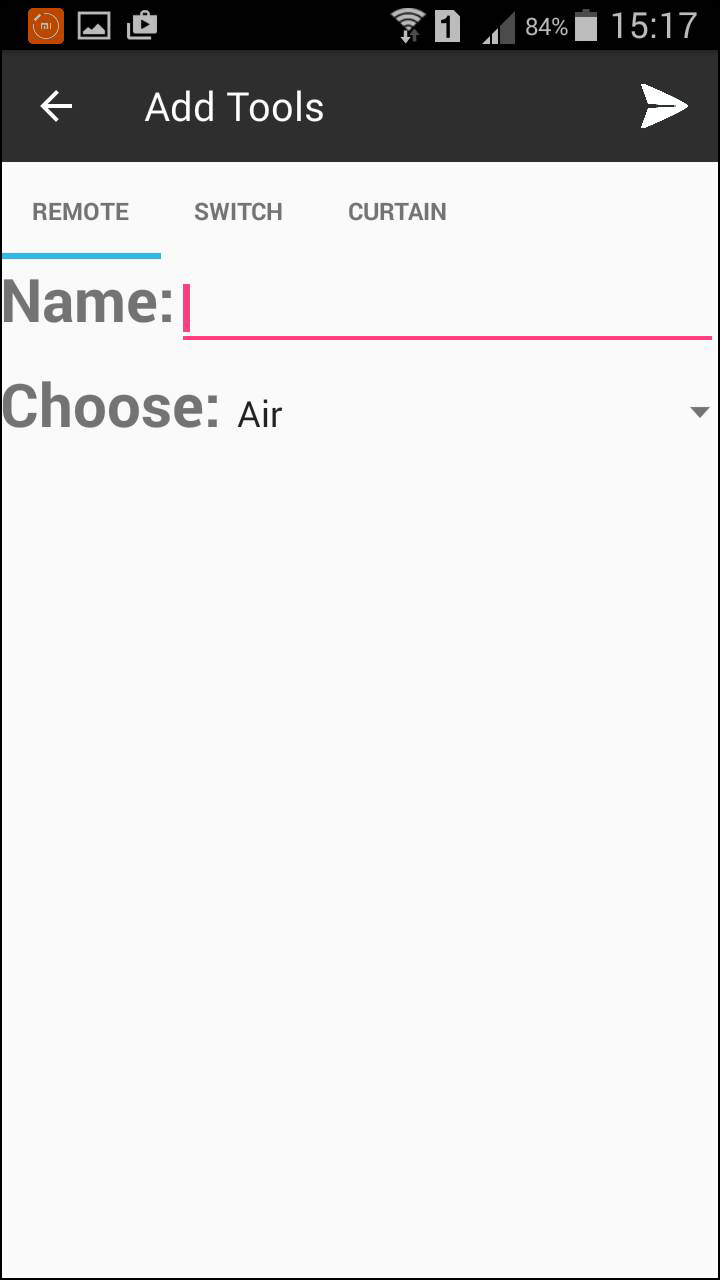
\includegraphics[width=0.27\textwidth]{addtool.jpg}
\caption{{\thi เพิ่มอุปกรณ์}}
\label{addtool}
\end{figure}
{\thi ซึ่งเมื่อกดเพิ่ม} {\thi แล้วจะแสดงอุปกรณ์ดังภาพ} 4.16 {\thi และเมื่อกดเมนูเพิ่มฉาก}(Add Scene) {\thi ก็แสดงดังภาพ} 4.17 {\thi ก็จะมีให้ใส่ชื่อของฉากและอุปกรณ์ที่ได้เพิ่มไว้ให้เลือก} 
 \newpage
\begin{figure}[h]
\centering
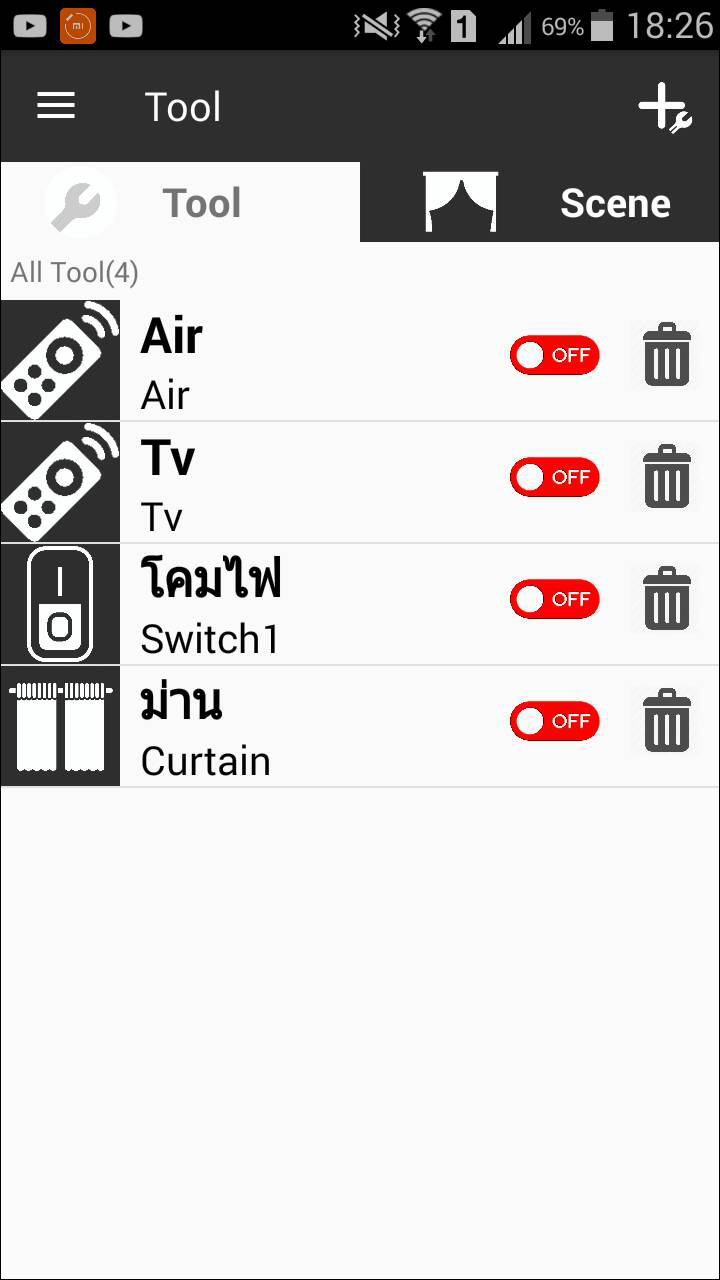
\includegraphics[width=0.27\textwidth]{showtoolpage.jpg}
\caption{{\thi แสดง} tool {\thi ที่เพิ่มไว้}}
\label{showtoolpage}
\end{figure}

\begin{figure}[h]
\centering
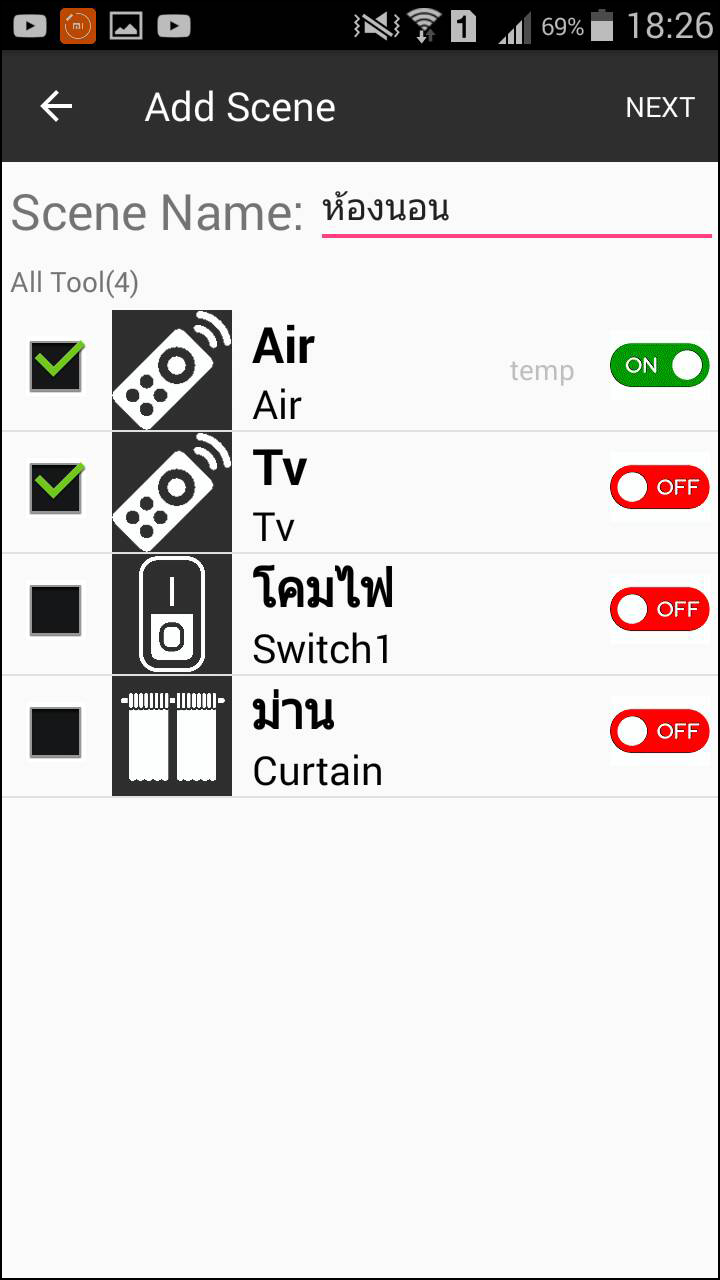
\includegraphics[width=0.27\textwidth]{addscenechoosetool.jpg}
\caption{{\thi ตั้งชื่อ}Scene,{\thi เลือก}tool}
\label{addscenechoosetool}
\end{figure}

{\thi เมื่อกด} next {\thi ก็จะไปหน้าที่ตั้งค่าของฉากดังภาพ} 4.18 {\thi ซึ่งมี} {\thi การตั้งเวลา}, {\thi ตั้งค่าเช็คอุณหภูมิ}, {\thi ตั้งค่าเช็คความเข้มแสงและตั้งค่าเช็คบลูทูธ} 
\newpage
\begin{figure}[h]
\centering
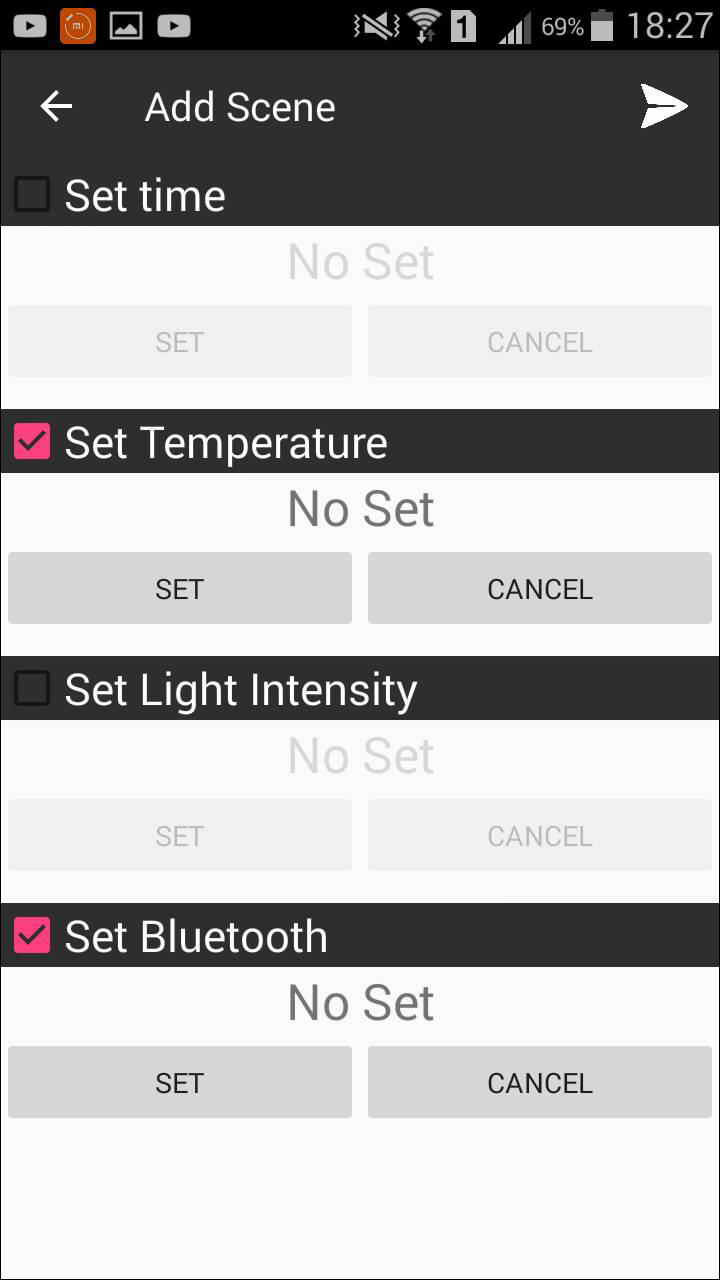
\includegraphics[width=0.27\textwidth]{setoptionscene.jpg}
\caption{Set option {\thi ของ} Scene}
\label{setoptionscene}
\end{figure}

{\thi ซึ่งเมื่อกด} set time {\thi จะแสดงดังภาพ} 4.19 {\thi โดยสามารถตั้งเวลาเป็นแบบ} 24Hours {\thi และกำหนดแบบรายสัปดาห์ได้} 

\begin{figure}[h]
\centering
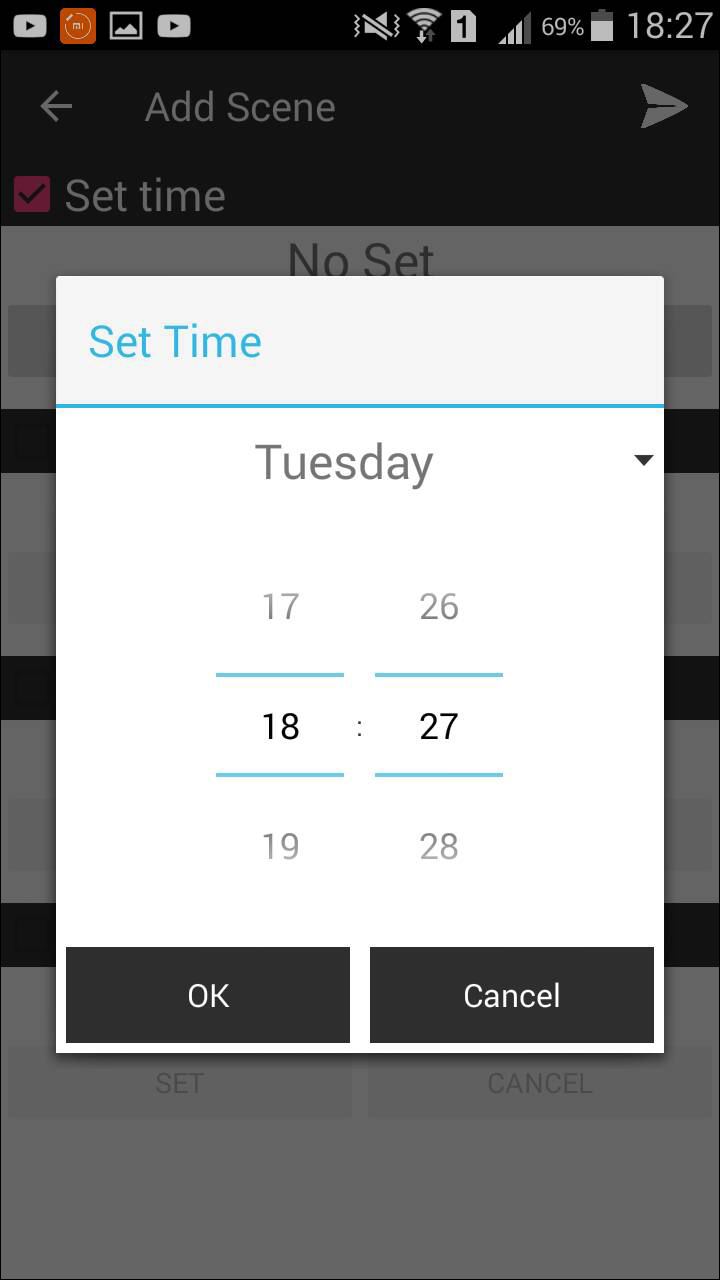
\includegraphics[width=0.27\textwidth]{settime.jpg}
\caption{Set Time}
\label{settime}
\end{figure}

\newpage
{\thi และเมื่อกด} set temperature {\thi ก็จะแสดงดังภาพ} 4.20 {\thi โดยจะให้ใส่เลขอุณหหมิ} {\thi และรูปแบบ} {\thi มากกว่า} {\thi หรือ} {\thi น้อยกว่ากว่าเท่ากับ}
\begin{figure}[h]
\centering
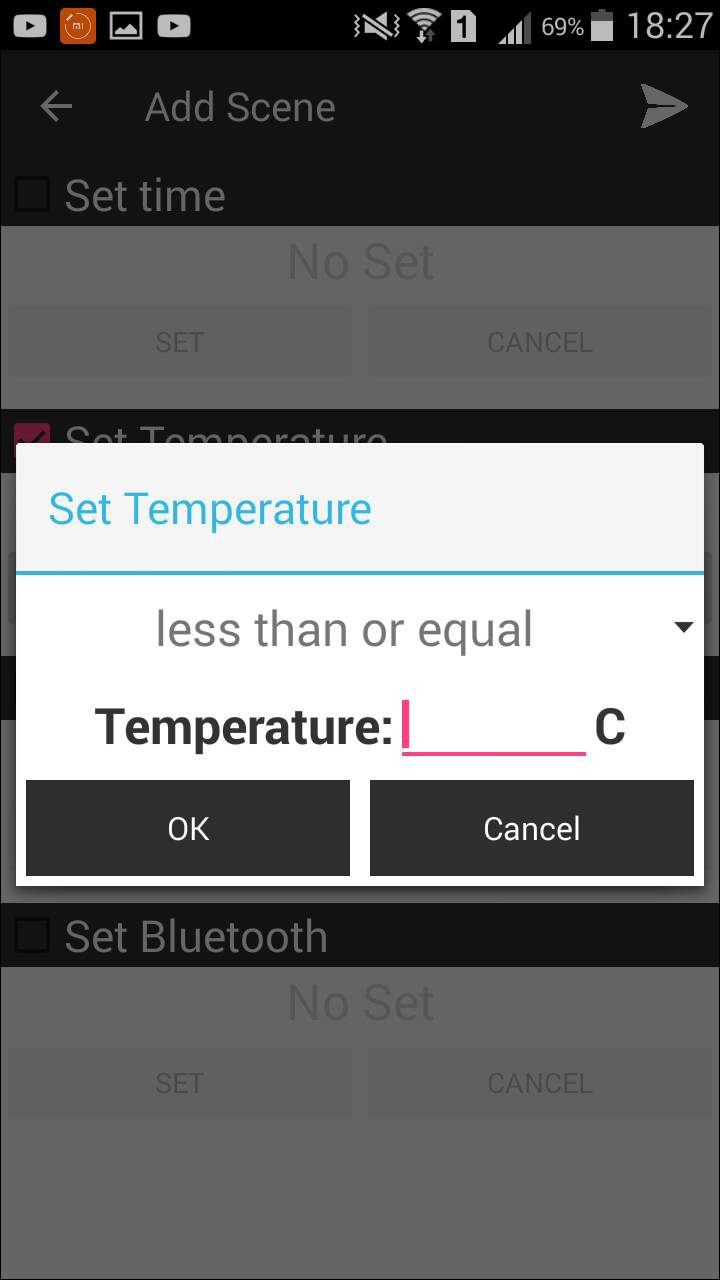
\includegraphics[width=0.27\textwidth]{settemp.jpg}
\caption{Set Temperature}
\label{settemp}
\end{figure} 

{\thi และเมื่อกด} set light intensity {\thi ก็จะแสดงดังภาพ} 4.21 {\thi โดยจะให้ใส่เลขความสว่าง} {\thi และรูปแบบ} {\thi มากกว่า} {\thi หรือ} {\thi น้อยกว่ากว่าเท่ากับ}
\begin{figure}[h]
\centering
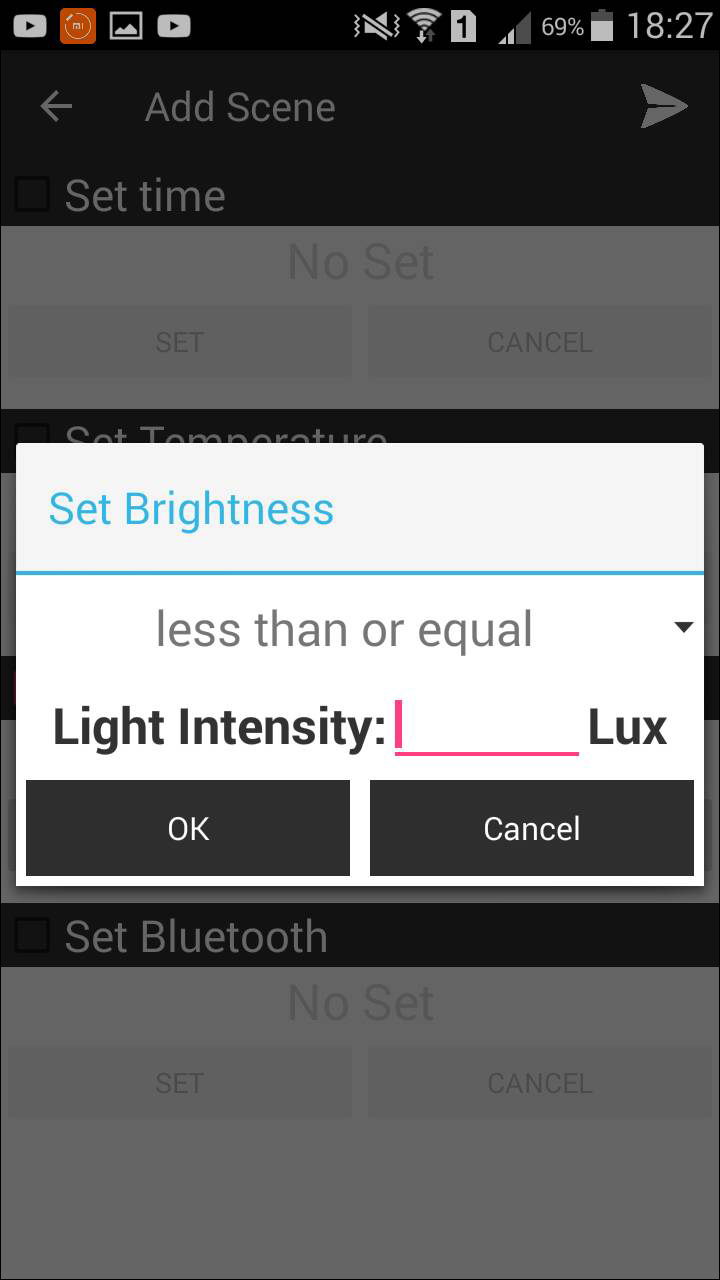
\includegraphics[width=0.27\textwidth]{setlight.jpg}
\caption{Set Brightness}
\label{setlight}
\end{figure} 

{\thi และเมื่อกด} set Bluetooth {\thi ก็จะแสดงดังภาพ} 4.22 {\thi โดยจะให้เลือกว่า} {\thi เมื่อเปิด} {\thi หรือปิดได้} {\thi จากนั้นเมื่อกดสร้างแล้ว} {\thi จะแสดง} {\thi ข้อมูลฉาก} {\thi ดังภาพ} 4.23
\newpage
\begin{figure}[h]
\centering
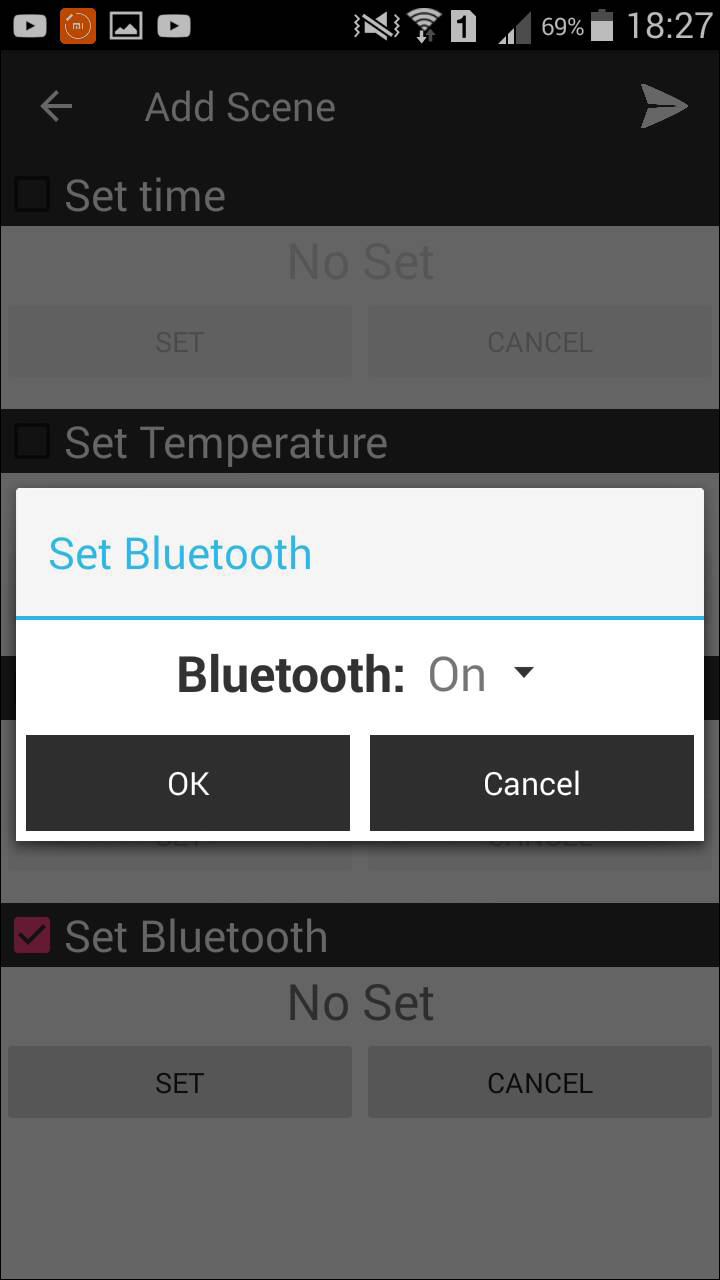
\includegraphics[width=0.27\textwidth]{setblue.jpg}
\caption{Set Bluetooth}
\label{setblue}
\end{figure}
\begin{figure}[h]
\centering
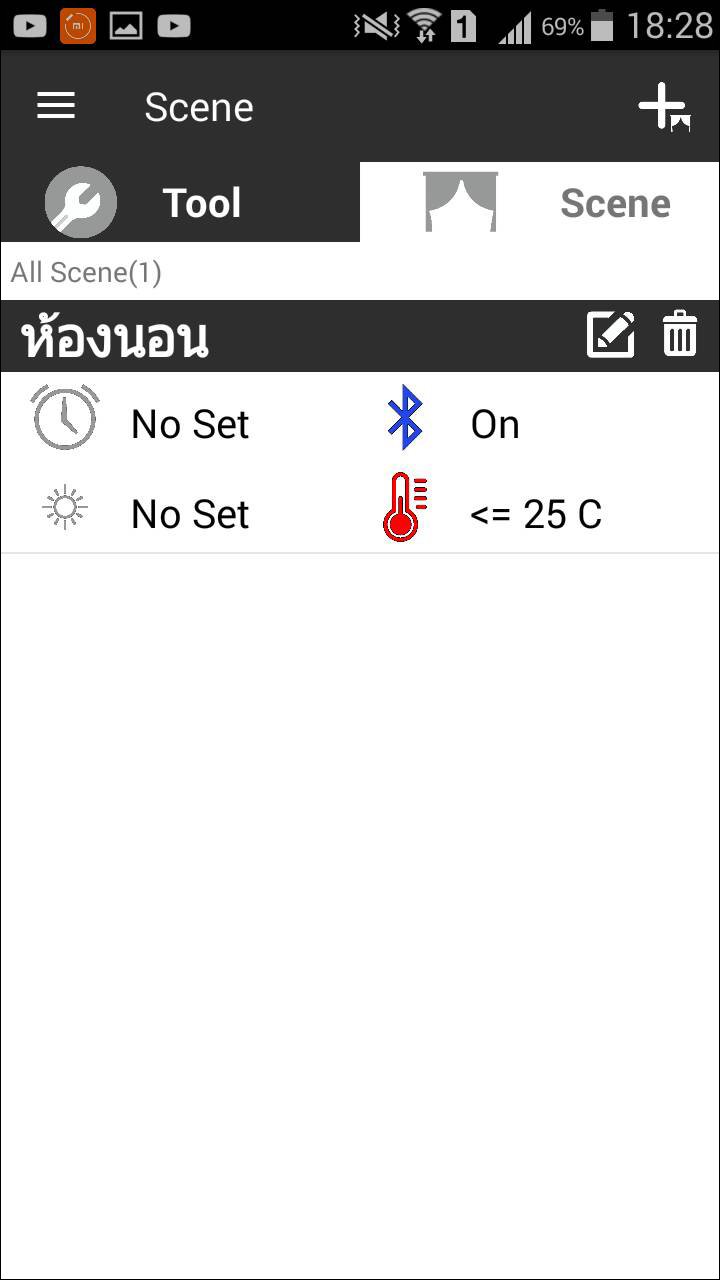
\includegraphics[width=0.27\textwidth]{showscene.jpg}
\caption{{\thi แสดง} scene {\thi ที่เพิ่มไว้}}
\label{showscene}
\end{figure}

{\thi เมื่อกดเมนูเพิ่ม} Bluetooth Address(Add Bluetooth Address) {\thi ซึ่งระบบจะทำการเช็คได้เพียงแค่ทีละ} 1 {\thi เครื่องเท่านั้น} {\thi การกดเพิ่มจึงเป็นการเซต} Bluetooth address {\thi ให้ระบบเช็คเครื่องของผู้ใช้นั้น} {\thi ดังภาพ} 4.24

\begin{figure}[h]
\centering
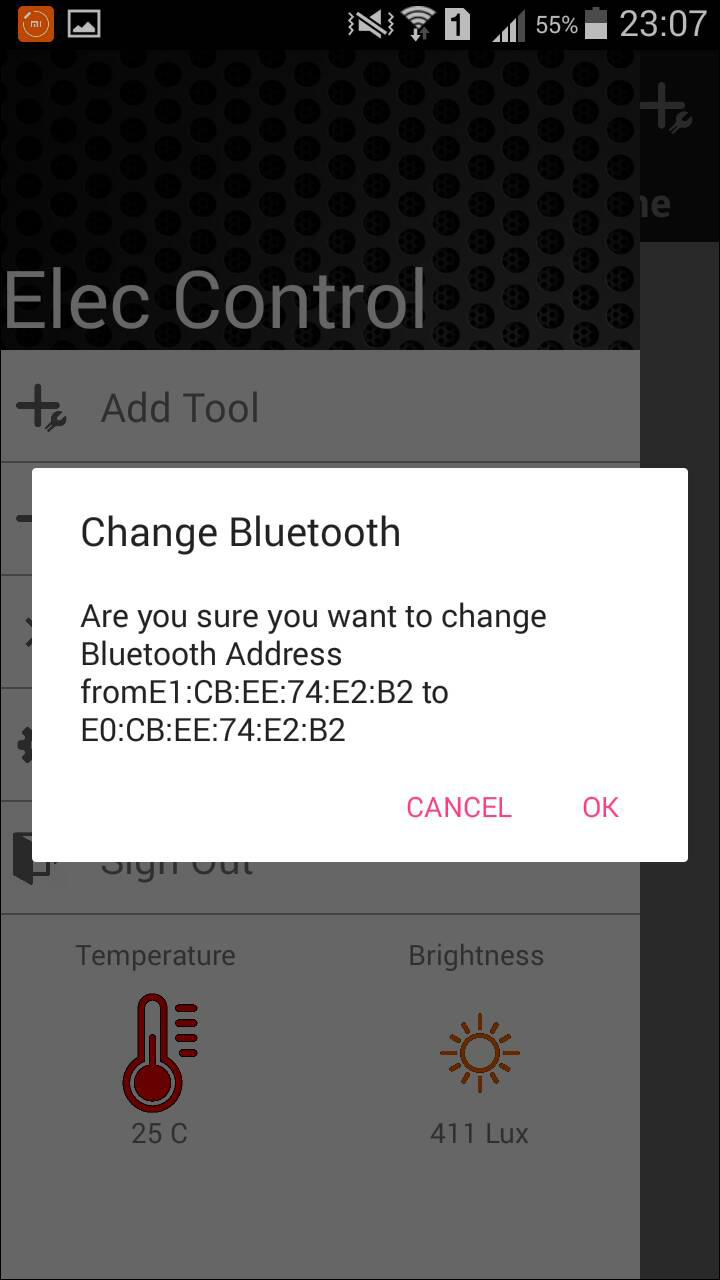
\includegraphics[width=0.27\textwidth]{setbluemac.jpg}
\caption{Set Mac Bluetooth}
\label{setbluemac}
\end{figure}
\newpage
{\thi เมื่อกดเมนูตั้งค่า} IP address (Set IP Address) {\thi จะแสดงดังภาพ} 4.25 {\thi โดยจะมีช่องให้ใส่เลข} IP {\thi เพื่อเชื่อมต่อเว็บเซอร์วิสของระบบ}
\begin{figure}[h]
\centering
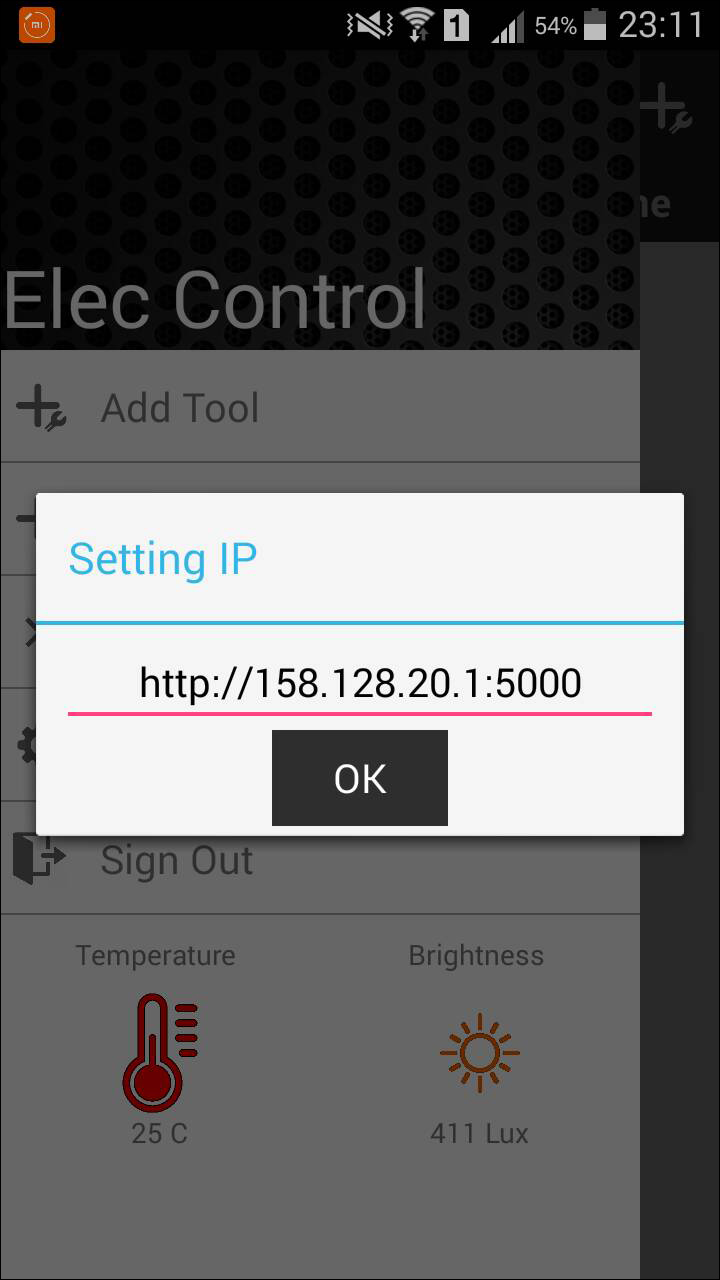
\includegraphics[width=0.27\textwidth]{setip.jpg}
\caption{{\thi แก้ไข} IP}
\label{setip}
\end{figure}

{\thi เมื่อกดเมนูตั้งค่า} Voice {\thi จะแสดงดังภาพ} 4.26 {\thi โดยจะมีหน้าต่างขึ้นมาเพื่อรอรับเสียงจากผู้ใช้}
\newpage
\begin{figure}[h]
\centering
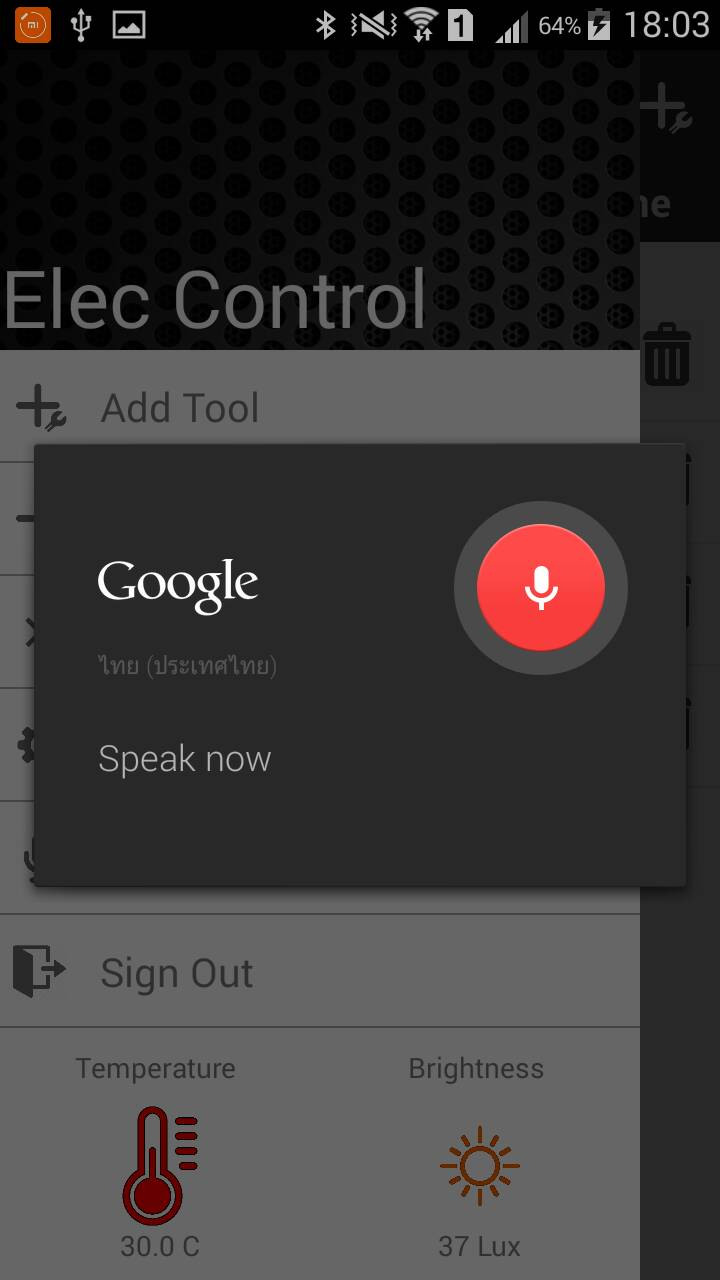
\includegraphics[width=0.27\textwidth]{voice2.jpg}
\caption{{\thi สั่งด้วยเสียง}}
\label{Voice}
\end{figure}

\subsection{{\thi การทดสอบวัดความพึงพอใจ}}
{\thi การทดสอบเพื่อวัดความพึงพอใจของผู้ใช้งานทั่วไป} {\thi ในการเข้าใช้งาน} {\thi ระบบควบคุม} {\thi เครื่องใช้ไฟฟ้าภายในบ้านผ่านแอปพลิเคชัน} {\thi การทดสอบจากผู้ใช้งานดังกล่าวนั้น} {\thi ได้แบ่งความพึงพอใจออกเป็น} 3 {\thi ด้าน} {\thi คือ}  
\begin{enumerate}
\item{{\thi ด้านการออกแบบ}}
\item{{\thi ด้านของการเลือกใช้เทคโนโลยีพัฒนาระบบ}}
\item{{\thi ด้านการทำงานของระบบ}}
\end{enumerate}

{\thi เครื่องมือที่ใช้ทดสอบ} {\thi คือ} {\thi แบบสอบถาม} {\thi ดังแสดงไว้ในภาคผนวก} {\thi ก} {\thi แบบประเมินความ} {\thi พึงพอใจทั้ง} 3 {\thi ตอนนี้} {\thi จะกำหนดภาพแบบของการประเมินความพึงพอใจแบบมาตราส่วนประมาณ} (rating scale) {\thi และกำหนดระดับความคิดเห็นออกเป็น} 5 {\thi ระดับ} {\thi ดังต่อไปนี้}   
\begin{itemize}
\item{5  {\thi หมายถึง}  {\thi ผู้ทดสอบมีความพึงพอใจมาก}}
\item{4  {\thi หมายถึง}  {\thi ผู้ทดสอบมีความพึงพอใจค่อนข้างมาก}}
\item{3  {\thi หมายถึง}  {\thi ผู้ทดสอบมีความพึงพอใจปานกลาง}}
\item{2  {\thi หมายถึง}  {\thi ผู้ทดสอบมีความพึงพอใจค่อนข้างน้อย}}
\item{1  {\thi หมายถึง}  {\thi ผู้ทดสอบมีความพึงพอใจน้อย}}
\end{itemize}

{\thi สำหรับเกณฑ์ที่ใช้ในการประเมินความพึงพอใจ} {\thi มีดังนี้} 
\begin{itemize}  
\item{4.50 {\thi –} 5.00  {\thi หมายถึง}  {\thi ความพึงพอใจมาก}}
\item{3.50 {\thi –} 4.49  {\thi หมายถึง}  {\thi ความพึงพอใจค่อนข้างมาก}}
\item{2.50 {\thi –} 3.49  {\thi หมายถึง}  {\thi ความพึงพอใจปานกลาง}}
\item{1.50 {\thi –} 2.49  {\thi หมายถึง}  {\thi ความพึงพอใจค่อนข้างน้อย}}
\item{1.00 {\thi –} 1.49  {\thi หมายถึง}  {\thi ความพึงพอใจน้อย}}
\end{itemize}
{\thi สถิติที่ใช้ในการวัดความพึงพอใจ} {\thi คือ} {\thi ค่าเฉลี่ย} (Mean)       

\section{{\thi ผลการทดลอง}}
	{\thi ผลการทดลองนำเสนอออกเป็น} 2 {\thi ส่วน} {\thi คือ} {\thi ส่วนแรกการทดสอบเพื่อวัดการทำงานของ} {\thi ระบบ} {\thi และส่วนที่สองการทดสอบเพื่อวัดพึงพอใจของผู้ใช้งานทั่วไป} (user)  

	{\thi การทดสอบเพื่อวัดการทำงานของระบบ} {\thi ทดสอบเพื่อตรวจหาข้อผิดพลาดการทำงาน} {\thi ในแต่ละส่วนของระบบก่อนที่จะนำไปใช้งานจริงโดยการทดสอบวัดการทำงานนั้น} {\thi แบ่งออกเป็น} 2 {\thi ส่วนคือ} {\thi ส่วนของระบบปฏิบัติการแอนดรอยด์} {\thi และระบบปฏิบัติการไอโอเอส} {\thi รายละเอียดดังตารางที่} 4.1 {\thi และ} {\thi ตารางที่} 4.2 {\thi โดยผลการทดสอบการทำงานของโปรแกรมในส่วนของระบบปฏิบัติการแอนดรอยด์} {\thi จะมี} 5 {\thi หน้าที่} {\thi คือ} {\thi การสร้างชุดคำสั่ง}  {\thi การตั้งระบบ} {\thi บลูทูธ} {\thi การตั้งระบบเซนเซอร์ต่าง} {\thi ๆ}  {\thi การสั่งการควบคุมอุปกรณ์ในระบบ} {\thi และการสั่งการตั้งเวลาควบคุม} {\thi อุปกรณ์ในระบบ} {\thi ซึ่งผลการทดลองการทำงานนั้นสามารถทำงานได้ดีตามวัตถุประสงค์ที่ตั้งไว้} {\thi ต่อมาเป็นผลการทดสอบการทำงานของอุปกรณ์ในส่วนของระบบปฏิบัติการไอโอเอสจะมี} 3 {\thi หน้าที่} {\thi การสร้างชุดคำสั่ง} {\thi การสั่งการควบคุมอุปกรณ์ในระบบ} {\thi และการสั่งการตั้งเวลาควบคุม} {\thi ซึ่งผลการทดสอบทั้งหมดสามารถทำงานได้ถูกต้องตามวัตถุประสงค์ที่ตั้งไว้}

	{\thi ส่วนการทดสอบความพึงพอใจของผู้ใช้งานทั่วไป}  {\thi ได้ทำการทดสอบจากความ}     {\thi พึงพอใจของผู้ใช้ระบบ} {\thi โดยจะแบ่งออกเป็น} 3 {\thi ด้าน} {\thi คือ} {\thi ด้านการออกแบบระบบ} {\thi ด้านการเลือกใช้เทคโนโลยีพัฒนาระบบ} {\thi และด้านการใช้งาน} {\thi ทดสอบโดยผู้ใช้ทำการใช้งานในส่วนต่าง} {\thi ๆ} {\thi ของระบบ} {\thi แล้วประเมินผลโดยการทำแบบสอบถามการใช้งาน} {\thi จากผู้ใช้} {\thi แล้วคำนวณค่าเฉลี่ยจากเกณฑ์ที่ได้}     {\thi ในการทำแบบสอบถามทั้งหมดโดยใช้สูตรค่าเฉลี่ย} (mean) {\thi ดังตารางที่} 4.3   

\begin{table}[h]
\centering
\caption{{\thi ผลการทดสอบแอปพลิเคชันในระะบบปฏิบัติการแอนดรอยด์}}
\label{and}\begin{tabular}{| l | c | l |}
\hline
\multicolumn{1}{|c|}{\textbf{{\thi หน้าที่การทำงาน}}} & \multicolumn{1}{l|}{\textbf{{\thi ทำได้}}} & \textbf{{\thi ทำไม่ได้}} \\ \hline
1.{\thi การเชื่อมต่อเข้าสู่ระบบ}                      & \#                                  &                   \\ \hline
2.{\thi แสดงการควบคุม} {\thi เปิด}/{\thi ปิดอุปกรณ์ในระบบ}          & \#                                  &                   \\ \hline
3.{\thi ตั้งเวลาควบคุมอุปกร์ในระบบ}                   & \#                                  &                   \\ \hline
4.{\thi สร้างชุดคำสั่ง}                               & \#                                  &                   \\ \hline
5.{\thi การทำงานอัตโนมัติโดยใช้} Sensor               & \#                                  &                   \\ \hline
\end{tabular}
\end{table}

\begin{table}[h]
\centering
\caption{{\thi ผลการทดสอบแอปพลิเคชันในระะบบปฏิบัติการไอโอเอส}}
\label{and}\begin{tabular}{| l | c | l |}
\hline
\multicolumn{1}{|c|}{\textbf{{\thi หน้าที่การทำงาน}}} & \multicolumn{1}{l|}{\textbf{{\thi ทำได้}}} & \textbf{{\thi ทำไม่ได้}} \\ \hline
1.{\thi การเชื่อมต่อเข้าสู่ระบบ}                      & \#                                  &                   \\ \hline
2.{\thi แสดงการควบคุม} {\thi เปิด}/{\thi ปิดอุปกรณ์ในระบบ}          & \#                                  &                   \\ \hline
3.{\thi ตั้งเวลาควบคุมอุปกร์ในระบบ}                   & \#                                  &                   \\ \hline
4.{\thi สร้างชุดคำสั่ง}                               & \#                                  &                   \\ \hline
\end{tabular}
\end{table}

\begin{table}[h]
\centering
\caption{{\thi ผลการประเมินความพึงพอใจของผู้ใช้งานทั่วไป}}
\label{and}\begin{tabular}{| l | c | c |}
\hline
\multicolumn{1}{|c|}{\textbf{{\thi รายงานประเมิน}}} & \textbf{{\thi ระดับคะแนนเฉลี่ย}} & \textbf{{\thi ระดับความพึงพอใจ}} \\ \hline
1.{\thi ด้านการออกแบบ}                              & 3.43                      & {\thi ปานกลาง}                   \\ \hline
2.{\thi ด้านการเรื่องใช้เทคโนโลยีของระบบ}           & 4.21                      & {\thi ค่อนข้างมาก}               \\ \hline
3.{\thi ด้านการทำงาน}                               & 3.74                      & {\thi ค่อนข้างมาก}               \\ \hline
\end{tabular}
\end{table}

\section{{\thi ปัญหาและอุปสรรค}}
\begin{itemize}
\item{{\thi อินเตอร์เน็ตช้า} {\thi ทำให้การควบคุมเครื่องใช้ไฟฟ้าไม่เป็นไปตามที่ต้องการ}}
\item{{\thi อุปกรณ์ด้านฮาร์ดแวร์มีปัญหา} {\thi เช่น} {\thi สายไฟหลวม}, {\thi สายไฟขาด},  nrf24i01 {\thi การส่งข้อมูลติดขัด}  ,IR Transmitter {\thi ส่งสัญญาณ} {\thi อินฟาเรด} {\thi ได้ระยะสั้น}}

\end{itemize}

\section{{\thi วิจารณ์}}
{\thi จากการทดสอบแอปพลิเคชั่นทั้ง} 2 {\thi ระบบปฏิบัติการ} {\thi ไอโอเอสและแอนดรอยด์} {\thi เป็นที่น่าพอใจ} {\thi เนื่องจากไม่พบข้อผิดพลาดในการทำงาน} {\thi แต่จะมีในบางครั้งที่เกิดการหน่วงช้าในการทำการจากความเร็วของอินเตอร์เน็ตของผู้ใช้งานหรือเซิร์ฟเวอร์}  {\thi ส่วน} Raspberry PI {\thi หากใช้งานพร้อม} {\thi ๆ} {\thi กันทั้งเซิร์ฟเวอร์และประมวลผลข้อมูลมาก} {\thi ๆ} {\thi จะทำให้ประสิทธิภาพในการทำงานลดลง}  


%%%%%%%%%%%%%%%%% {\thi สรุป} %%%%%%%%%%%%%%%%%%%
\chapter{{\thi สรุป}}


\section{{\thi สรุป}}
	{\thi โครงการฉบับนี้เสนอระบบควบคุมเครื่องใช้ไฟฟ้าภายในบ้านผ่านแอปพลิเคชั่น}
{\thi โดยพัฒนาในภาพแบบโมบายแอพพลิเคชั่น} (mobile application) {\thi เครื่องมือที่ใช้พัฒนา} {\thi คือ}
{\thi โปรแกรม} android studio   , python , java {\thi และ} JavaScript{\thi โดยมี} {\thi วัตถุประสงค์หลักของการพัฒนาคือ} {\thi เพิ่มช่องทางการควบคุมอุปกรณ์ไฟฟ้าภายในบ้าน}  {\thi โดยใช้โทรศัพท์เคลื่อนที่ที่ใช้ระบบปฏิบัติการแอนดรอยด์} {\thi และ} {\thi ระบบปฏิบัติการไอโอเอสโดยที่ผู้ใช้งานสามารถควบคุมการทำงานของระบบ} {\thi ได้จากแอปพลิเคชั่นนี้} {\thi ด้วยการเชื่อมต่อเครือข่ายอินเตอร์เน็ต} {\thi การสั่งควบคุมการเปิดหรือปิดอุปกรณ์ไฟฟ้าภายในระบบ} {\thi ตั้งเวลาการเปิดหรือปิดอุปกรณ์ไฟฟ้าภายในระบบได้} {\thi และเมื่อพัฒนาเสร็จได้ทำการทดสอบประสิทธิภาพโดยผู้พัฒนา} {\thi โดยตรวจสอบแบ่งออกเป็น} 2 {\thi ส่วน} {\thi คือ} {\thi ส่วนของแอปพลิเคชั่นควบคุมว่าสามารถสั่งการได้อย่างสมบูรณ์หรือไม่} {\thi ผ่านโทรศัพท์มือถือประเภทสมาร์ทโฟน}  {\thi และส่วนต่อมาคือส่วน} {\thi ของวงจรควบคุมระบบภายในที่สามารถตอบสนองต่อการควบคุม} {\thi และทำงานได้อย่างถูกต้องตาม} {\thi กำหนดหรือไม่} {\thi อย่างไรก็ตาม} {\thi การทำงานสั่งการของ}    {\thi แอปพลิเคชั่นนั้นยังไม่รวดเร็วมากนัก} {\thi ในช่วงเวลาระหว่างการสั่งการทำงานนั้นต้องใช้การหน่วงเวลาชั่ว} {\thi ครู่จึงจะทำงานได้ตามการควบคุม}

\section{{\thi ข้อเสนอแนะ}}
	{\thi การพัฒนาระบบควบคุมเครื่องใช้ไฟฟ้าภายในบ้านผ่านแอปพลิเคชั่น}  {\thi กรณีศึกษาคณะวิศวกรรมศาสตร์ศรีราชา}  {\thi มหาวิทยาลัยเกษตรศาสตร์} {\thi วิทยาเขตศรีราชา}    {\thi สมาร์ทโฟน} {\thi สามารถนำไปใช้งานได้จริง} {\thi แต่ก็ยังสามารถพัฒนาเพิ่มเติมขีดความสามารถได้อีก} {\thi ซึ่งจะมี} {\thi การพัฒนาอย่างต่อเนื่องเช่นกัน} {\thi และนอกจากนี้ผู้จัดทำจึงขอเสนอแนะการเพิ่มเติมดังนี้}

	\begin{itemize}
	\item{{\thi การใช้}  Raspberry PI {\thi ในการใช้งานหลายๆอย่างพร้อมกันนั้น} {\thi ไม่ว่าจะเป็นเว็บเซิร์ฟเวอร์} {\thi การประมวลผลโปรแกรมต่างๆ}      {\thi ซึ่งใช้ทรัพยากรอย่างมากทำให้เกิดความล่าช้าในการทำงาน}}
	\item{{\thi โครงงานนี้มีกระแสไฟเลี้ยงขาเข้าเป็นไฟฟ้ากระแสสลับสูงถึง} 220v {\thi การพัฒนาต่อ} {\thi หรือการใช้งานจริงต้องมีความระมัดระวังในการดำเนินการเป็นอย่างดี}}
	\item{{\thi โครงการนี้} {\thi เป็นโครงการที่พัฒนาขึ้นเพื่อเป็นกรณีศึกษาของคณะวิศวกรรมศาสตร์ศรีราชา}  {\thi มหาวิทยาลัยเกษตรศาสตร์} {\thi วิทยาเขตศรีราชา} {\thi เท่านั้น} {\thi การพัฒนาในอนาคตควรจัดทำให้} {\thi โครงการนี้สามารถใช้งานโดยมีขอบเขต} {\thi และความสามารถในการทำงานที่สูงกว่านี้}}
	\end{itemize}



%%%%%%%%%%%%%%%%%%%%% References %%%%%%%%%%%%%%%%%%%%%%%
\newpage
\addcontentsline{toc}{chapter}{{\thi เอกสารและสิ่งอ้างอิง}}
\bibliographystyle{plain}
\bibliography{myprop_ref}

%%%%%%%%%%%%%%%%%%%%% Appendices %%%%%%%%%%%%%%%%%%%%%%%
\appendix
%%%%%%%%%%%%%%%%% {\thi คู่มือการติดตั้งโปรแกรม} %%%%%%%%%%%%%%%%%%%
\chapter{{\thi คู่มือการติดตั้งโปรแกรม}}
\section{Android}
\begin{enumerate}
\item{{\thi นำ} ElecControl.apk {\thi ไปไว้ในเครื่องโทรศัพท์ที่เป็นระบบปฏิบัติการ} Android {\thi ดังภาพที่} A.1}

\item{{\thi เมื่อขึ้นหน้าต่างดังภาพ} A.2 {\thi แล้วกด} install}

\item{{\thi สามารถใช้งานได้} {\thi ดังภาพ} A.3}

\end{enumerate}

\begin{figure}[h]
\centering
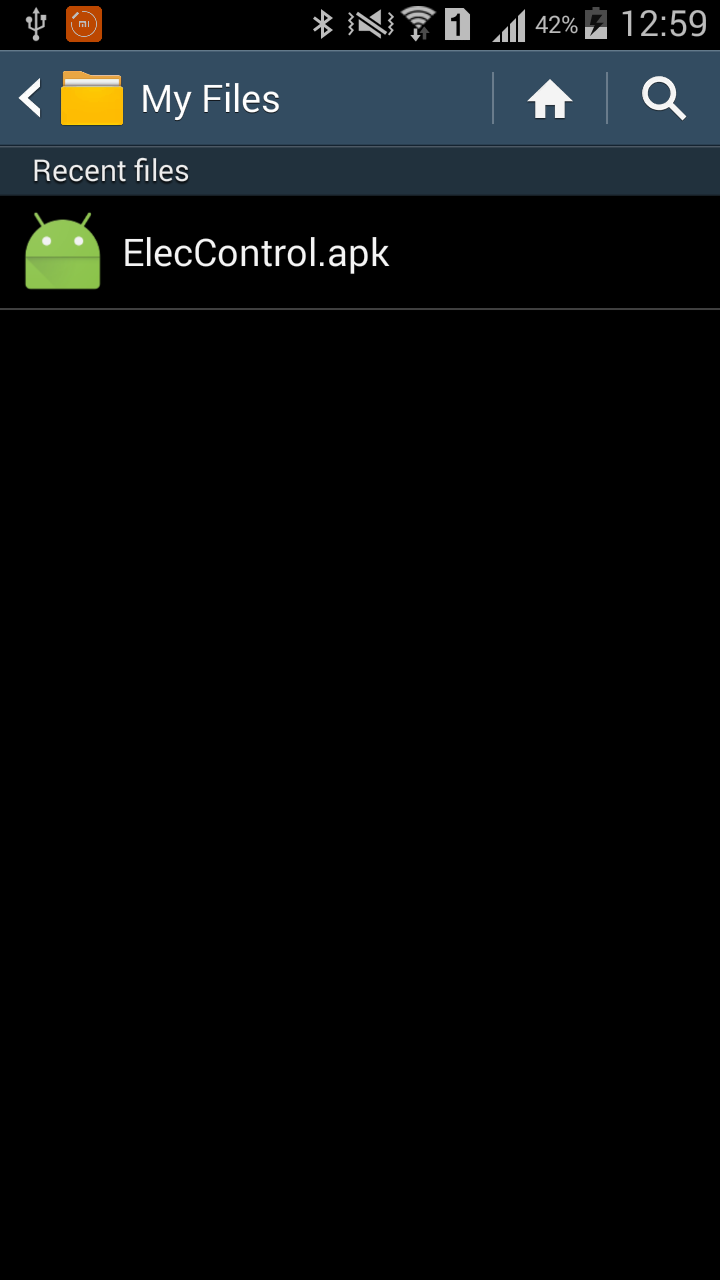
\includegraphics[width=0.25\textwidth]{and1.png}
\caption{ElecControl.apk}
\label{and1}
\end{figure}
\newpage
\begin{figure}[h]
\centering
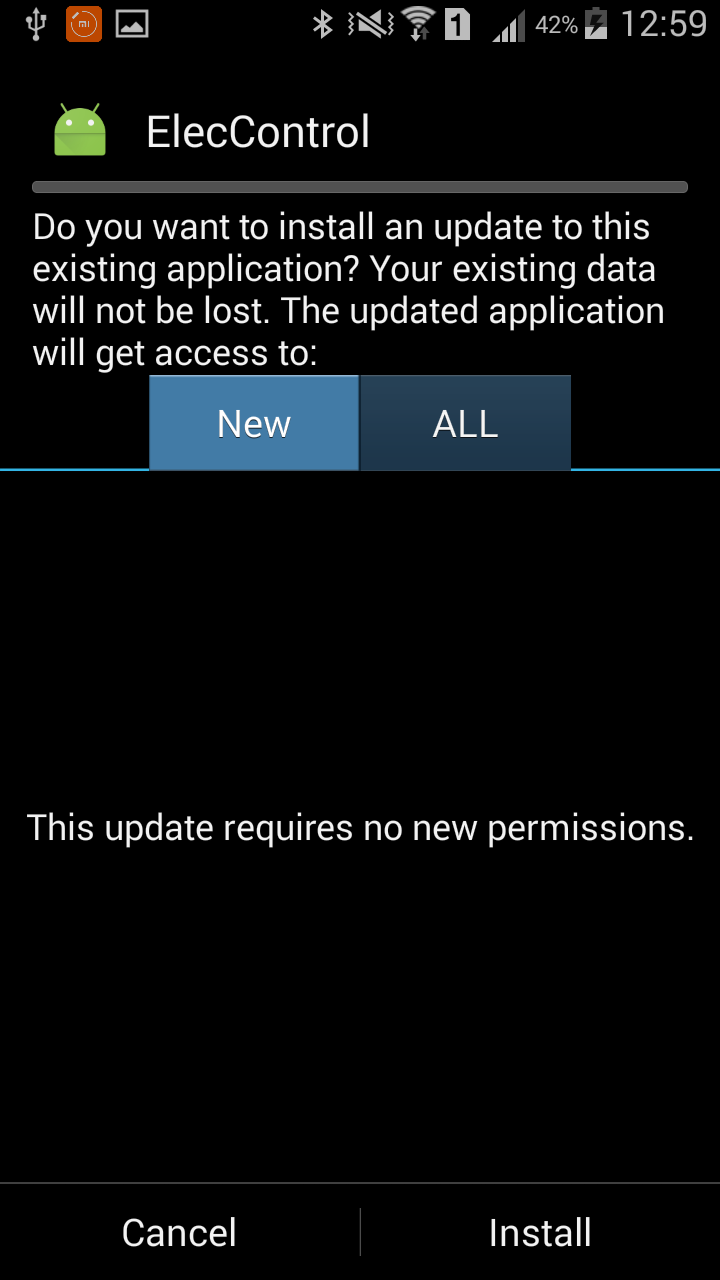
\includegraphics[width=0.25\textwidth]{and2.png}
\caption{install ElecControl}
\label{and2}
\end{figure}
\begin{figure}[h]
\centering
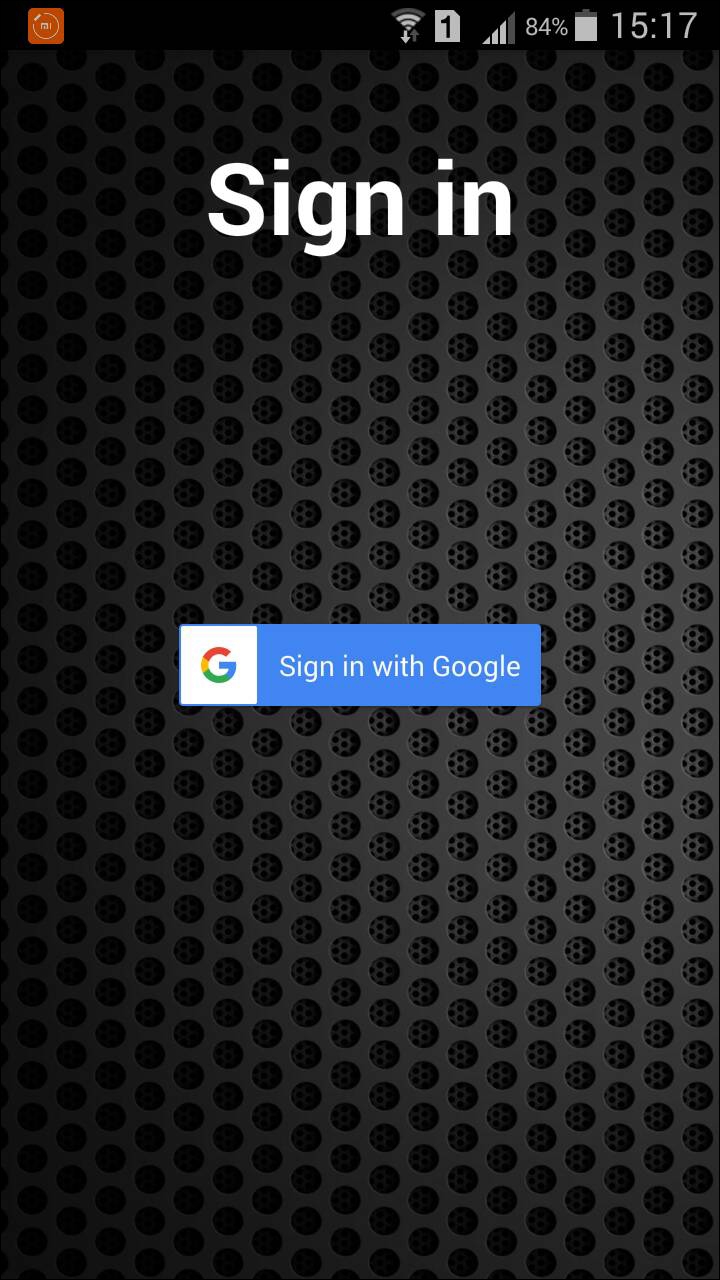
\includegraphics[width=0.25\textwidth]{and3.jpg}
\caption{Success install}
\label{and3}
\end{figure}
\newpage
\section{IOS}
\begin{itemize}
\item{Download application iDevices {\thi จาก} App Store {\thi หรือ} {\thi จะใช้}  Apple Homekit}
\end{itemize}
\section{Raspberry Pi3}
\subsection{install npm}
{\thi สามารถดูการติดตั้งได้ที่} \cite{HomeKit}

\subsection{install lirc}
{\thi สามารถดูการติดตั้งได้ที่} \cite{LIRC}

\subsubsection{{\thi ขั้นตอนที่} 2: run Core.js}

{\thi เปิด} command line {\thi แล้วไปที่} path /HAP-NodeJS

sudo node Core.js 

{\thi ตามภาพที่} A.4

\begin{figure}[h]
\centering
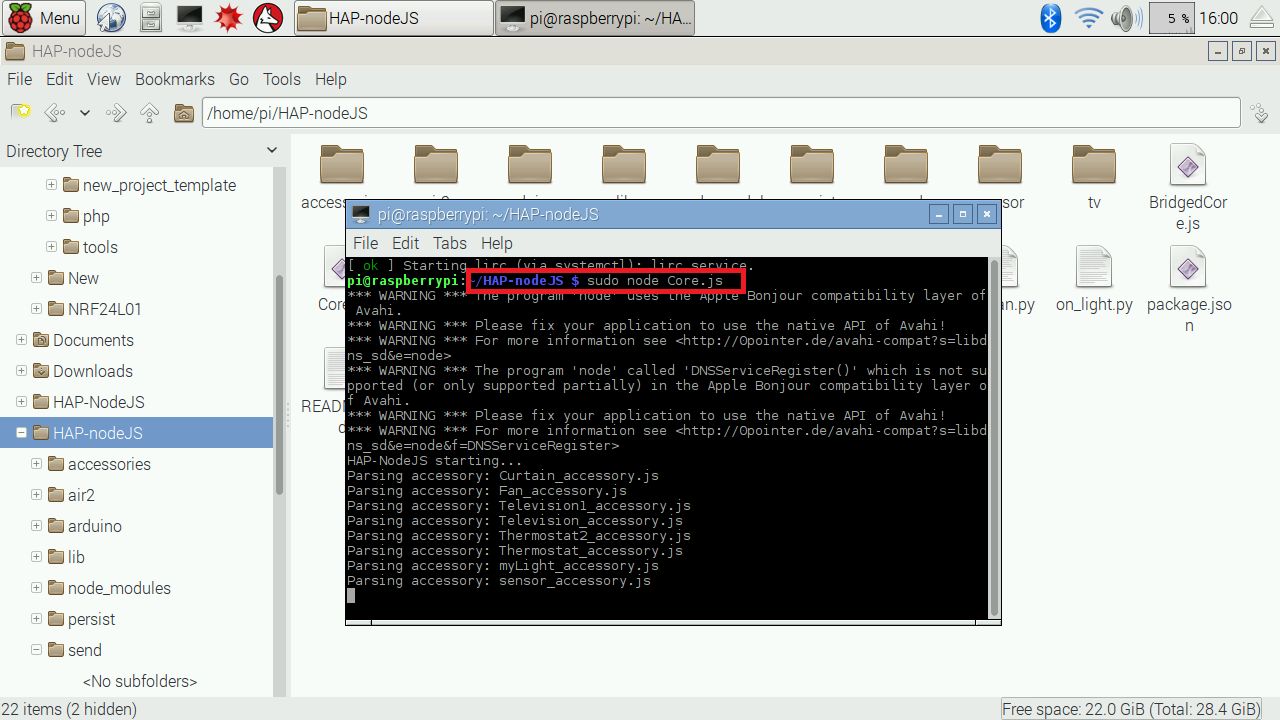
\includegraphics[width=0.9\textwidth]{cd5.png}
\caption{Core.js}
\label{cd5}
\end{figure}

\subsubsection{{\thi ขั้นตอนที่} 2: run web service}
{\thi เปิดไฟล์} web android.py {\thi ด้วย} python ver.3.5 {\thi แล้วกด} run {\thi ตามภาพที่} A.5

\begin{figure}[h]
\centering
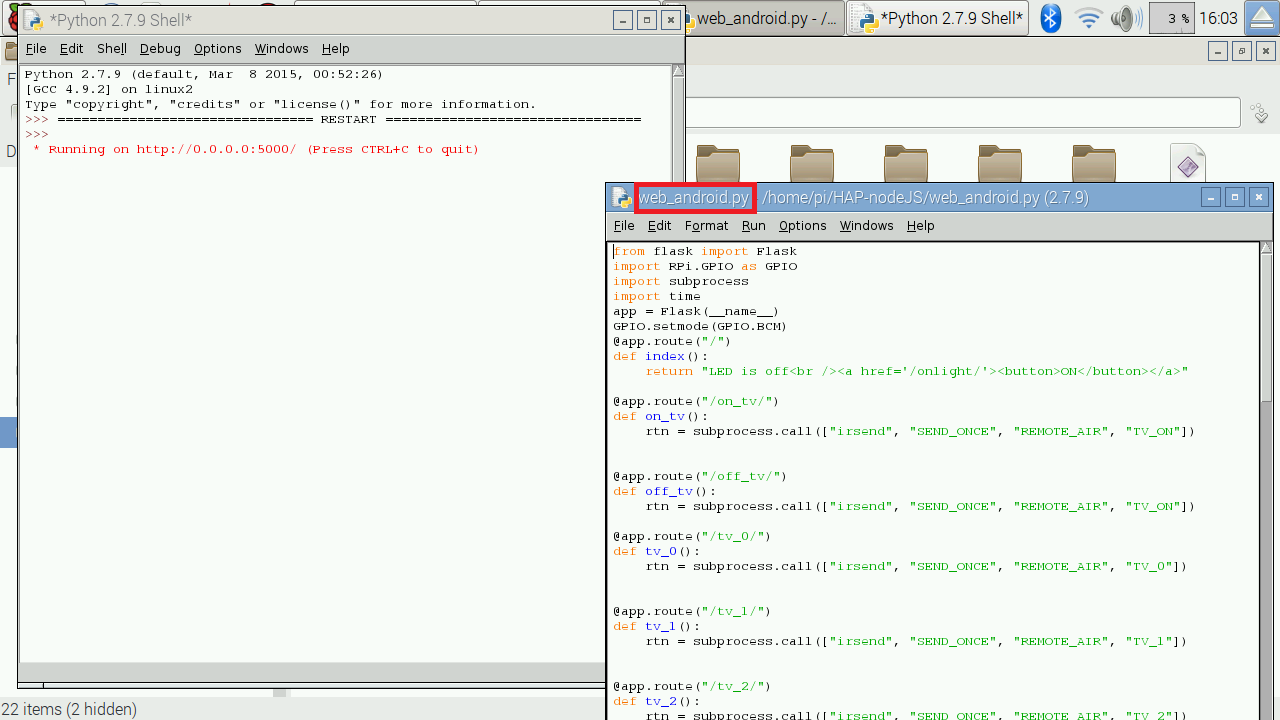
\includegraphics[width=0.9\textwidth]{cd6.png}
\caption{web android.py}
\label{cd6}
\end{figure}



}
\end{document}
%%%%%%%%%%%%%%%%%%%% Document Ending %%%%%%%%%%%%%%%%%%%%%
